\documentclass[12pt]{article}
\usepackage[utf8]{inputenc}

\usepackage[symbol]{footmisc} % footnote symbols

\usepackage{float} % force figure location with [H]
\usepackage{xcolor}

\usepackage{graphicx}
\graphicspath{ {output/} } % compile mode must be normal for images to display

% Customize figure captions
\usepackage{caption}
\captionsetup{font = {footnotesize, onehalfspacing}, labelfont = bf, textfont = it}

\usepackage[
    letterpaper, 
    portrait, 
    margin=1in]{geometry} % set paper size, orientation, and margins
    
\usepackage[
    backend=biber,
    style=apa]{biblatex} % Imports biblatex package
    
\addbibresource{ref.bib} % Import the bibliography file

% set line spacing
\setlength{\parindent}{3em}
\setlength{\parskip}{0em}
\renewcommand{\baselinestretch}{1.25}

\renewcommand{\thefootnote}{\fnsymbol{footnote}}




\begin{document}

\hspace{5pt}

\Large
 \begin{center}
Expanding the Coverage and Accuracy of Parcel-Level Land Value Estimates\footnote[2]{Gold and Binder acknowledge financial support from the David \& Lissa Leege Endowment and professional development grant funds from the Faculty Life Committee of St Olaf College. They would also like to thank Rushikesh Jadhav for research assistance and Sara Dale and Craig Rice for their indispensable technical assistance.}\\ 
% I need to verify that I'm acknowledging the funding sources properly.

\vspace{10pt}

% Authors
\large
Asa Gold$^1$, Seth Binder$^1$, Christoph Nolte$^2$ \\

\vspace{10pt}

\footnotesize  
$^{1}$St. Olaf College\\
$^2$Boston University

\vspace{40pt} 

    \normalsize
    \textbf{Abstract}
\end{center}

\small
Planning for cost-effective conservation requires reliable estimates of land costs, spatially-differentiated at high resolution. Nolte (2020) provides a county-by-county, parcel-level estimation approach that dramatically improves estimates of fair market value for undeveloped land across the contiguous Unites States. Much undeveloped land of conservation interest is under threat of conversion to agricultural use or is already agricultural. This paper demonstrates the value of accounting for additional variables that affect agricultural productivity and demand for undeveloped land, as well as the benefit of modeling at scales corresponding to regional agricultural markets. We find that countywide median home value, climatic variables, and several parcel-level soil type variables contribute substantially to predictive power. Enlarging the set of predictors and the geographical scale of modeling improves accuracy by approximately 13 percent and extends coverage into 376 counties occupying 1.35 million km$^2$.

\newpage

\section{Introduction}

Agencies and private organizations designing conservation efforts must contend with the fundamental scarcity of available resources, while simultaneously confronting a vast array of potential conservation strategies. Accurately predicting costs of competing strategies, then, is crucial to achieving the cost-effective use of scarce conservation dollars. The value of land is the primary determinant of such costs. Yet, academics and planners have not often had access to reliable estimates of fair market land value, which constitute a high-priority resource for global change science and policy in general (\cite{Coomes2018GeospatialPolicy}). Some studies of conservation cost have relied on state or county-wide average land value estimates (e.g., \cite{Withey2012MaximisingUSA}; \cite{Lawler2020PlanningConfiguration}),
which obscure important heterogeneity of land values across those geographically large political units. Recent work suggests that conservation strategies based on such low-resolution cost estimates can substantially underestimate the cost of selected plans (\cite{Nolte2020High-resolutionStates}). 

Several studies have attempted more accurate, higher-resolution land value estimates with national coverage. \textcite{Larson2015} uses a patchwork of USDA county-level agricultural land value estimates and existing hedonic estimates of urban land value (\cite{Kuminoff2013}) to interpolate values to a mix of parcels, census tracts, and counties across the contiguous U.S. \textcite{Albouy2018} estimate urban land values for every Metropolitan Statistical Area (MSA) in the U.S. For each MSA, they leverage sales data from the CoStar COMPS database to estimate land value per acre as a continuous function of distance from the city center. The majority of conservation interest, of course, lies outside of urban areas. With a primary focus on undeveloped land, Nolte (2020) integrates a nationwide database of parcel-specific information, including location, built environment, local demographics, and physical landscape features, with Zillow’s ZTRAX database of millions of sales records for use in a machine-learning algorithm to estimate land values at much higher spatial resolution. These estimates explain a much greater portion of observed variation in sales value than county-wide averages. The Nolte approach constitutes a leap forward for estimating the value of undeveloped land value for conservation planning. As we show here, it can be further improved.

There is reason to believe that expanding both the set of agriculturally and economically relevant predictors as well as the geographic scale of analysis could improve the coverage and quality of land value estimates. The market value of undeveloped land is in many cases driven by the value of its actual or potential use in agriculture. It can also be driven by demand in related, residential land markets. Climate and soil variables, absent from the set of \textcite{Nolte2020High-resolutionStates} predictors, are well known to be important determinants of agricultural productivity and land value. Irrigation can also be an important determinant of productivity for particular crops and geographies, though it requires costly investment. The irrigation status of land can indicate unobserved investments in machinery, infrastructure or physical changes to land that enhance its market value. 

While many of the land quality attributes that determine economic value are fixed, or change only very slowly over time, many drivers of supply and demand—income, preferences, technology, and the availability of substitutes---vary over time. Failing to account for time-varying predictors can lead to an erosion of predictive power. When sales prices exhibit trends over time, not only will overall estimation accuracy suffer but models might systematically over- or under-predict sales values for observations before or after the median sales year if they do not adequately control for such tends. To address these issues, we add median home price indices to our set of predictors. Home price indices capture changing dynamics in residential land markets that can exert pressure on (or otherwise correlate with) the price of undeveloped land. Accounting for variation in local home prices might thus improve the predictive power of models aimed at estimating the value of agricultural or other undeveloped land. 

Beyond incorporating additional predictors, we consider the possibility that modeling at scales larger than the county can ease local observation constraints, improving both the coverage and accuracy of resulting estimates. Many counties have few sales records in the ZTRAX database. Nolte (2020) implements a 1000-observation minimum for modeling parcel land values within a county, supplementing a focal county’s observations with observations drawn from neighboring counties where possible. In replicating this supplementation procedure with vacant, undeveloped, and agricultural parcels, we find that 27 percent of counties in the study sample fail to meet the threshold, and prediction accuracies for counties with sufficient-but-low observation densities are notably poorer than those for other counties. 

Indeed, national performance aggregations mask substantial heterogeneity across county characteristics. In particular, a county's observation density is strongly correlated with both performance measures. Figure \ref{fig:compare_county_nobs_perf} shows the relationship between model performance and the total number of observations in the county where the model was trained and tested. The monotonicity of the decrease (increase) in mean squared error (r-squared) as county-level models increase in size affirms the intuitive benefits of greater sample sizes. In pursuit of larger datasets, however, analysts will encounter a fundamental challenge: expanding the sample size necessarily broadens the geographic range from which observations will be drawn. This may debilitate the model's predictive power if the broader geographic scope mixes land markets with disparate characteristics, economic dynamics, and time trends. Yet failing to expand the geographic scope has its own costs. In states such as Wyoming and Idaho, any given county has too few observations to model land value, forcing the analyst to discard otherwise high quality data.

We attempt to solve this trade-off between model size and observation homogeneity by specifying models at the level of the farm resource region (Figure \ref{fig:FRR_map}). USDA farm resource regions are delineated in consideration of county-level, often cross-state similarities in geography and agricultural production (\cite{FRR2000}).

Overall, our modeling approach, which both expands the set of predictors and models at a regional scale, improves prediction error by 13 percent. Decomposing this effect, we see that adding variables alone (without modeling at a regional scale) reduces prediction error by 9 percent, while modeling at a regional scale \textit{further} reduces prediction error by 5 percent (based on common parcels modeled at both scales, using the full set of predictors). By modeling at the farm resource region level, we extend coverage in areas that were dropped in county modeling due to insufficient density by 376 counties while preserving comparable predictive accuracy to county-level approaches. In short, our approach enhances the quality and quantity of parcel-level estimates of fair market value. 


\section{Data and Methods}
We base our analysis on the approach first published by Nolte (2020), which trains a tree-based, ensemble learning algorithm on a comprehensive high-resolution dataset of parcel characteristics and sales across the contiguous United States (140.9 million properties across 3,055 counties) to estimate the logged, inflation-adjusted, per-hectare value of parcels lacking recent sales data. The present study uses extremely randomized trees, a decision tree-based bagging algorithm, with 500 base learners (trees), $\frac{p}{3}$ random features tried at each split, where $p$ is the total set of predictive features, and a required minimum leaf size of 3. Nolte (2020) estimates models for the group of all parcels greater than 1 acre in size as well as separate models for the subset of stringently defined ``vacant" (undeveloped) parcels. Parcels of interest in this study include all ``vacant'' parcels plus any additional parcels coded as agricultural, even if they contain a building footprint. Our filter (fully described in Appendix A.1) results in 5.04 million unique sales observations nationwide, split into testing (\textit{n = 1.26 million}) and training (\textit{n = 3.78 million}) sets balanced on the outcome variable (Fig. \ref{fig:clean_obs_density}). In county models, this 0.75:0.25 split occurs within the county; in farm resource region models, training and testing observations are distributed farm resource region-wide. For county-level models, counties with fewer than 1000 observations are augmented with randomly sampled sales from adjacent counties until the focal county reaches 1000 observations. If the county and its neighbors combined fail to achieve 1000 complete observations, no model is specified. 1,571 county models are specified using this approach.

Among the set of predictors in Nolte (2020) are variables on building presence, development, accessibility, local demographics, local nature preservation, terrain, water, land cover type, location, and date of sale. To these base data, we add variables for climate, irrigation status, soil quality, and local real estate prices.\footnote{Our predictor set is missing two flood risk variables used in Nolte (2020).} Our climate variables are 30-year, climate normals of monthly minimum, mean, and maximum temperature, as well as dew temperature and precipitation from the PRISM Climate Group (\cite{PRISMClimate2021}). We aggregate these to the meteorological season. Parcel irrigation status is based on annual 1997-2017 estimates at a resolution of 30 sq. meters, produced by the Landsat-based Irrigation Dataset, or LANID-US (\cite{Xie2021MappingStates}). We create two binary irrigation variables to record 1) whether the parcel had ever been irrigated prior to sale, and 2) whether it was irrigated at any point in the 3 years immediately preceding the sale. 

Soil classifications, indicating a map unit's suitability for agricultural use, were compiled from the Natural Resources Conservation Service (NRCS)’s high-resolution SSURGO soil survey database (\cite{SoilSurveyStaffSoilStates}). The NRCS soil survey provides map unit polygons that describe soil components (e.g., ``loamy fine sand, 0 to 2 percent slopes") and characteristics, including water capacity, flooding frequency, farmland classification, and features limiting development, among others. Soil farmland classifications, indicating a map unit's suitability for agriculture, fall under five general classes, defined by the USDA:
\begin{enumerate}
    \item Prime, optimal site composition and availability for producing agricultural product;  
    \item Unique, soil producing high-value crops (e.g., vineyards in California); 
    \item Statewide Importance, state-defined agricultural land that fails to meet prime criteria;
    \item Local importance, locally defined agricultural land that fails to meet prime or statewide criteria
    \item Conditional classes, land that would be considered prime, of statewide importance, or of local importance conditional on a specified improvement (e.g., ``Prime if drained and protected from flooding")
\end{enumerate}

Farmland classifications are operationalized as the percent of each parcel containing a given classification (e.g., ``Prime Farmland” or ``Farmland of Statewide Importance”). Aggregation is applied to overlapping classifications containing multiple conditions. For instance, ``Prime if drained or protected from flooding" gets assigned to ``Prime if drained" and ``Prime if protected from flooding." For sales records covering multiple parcels, our soil aggregation strategy is described in Appendix A.3. 

To incorporate information on local real estate markets, we add yearly all-transaction house price index values at the county level (\cite{FederalHousing2022}). At the farm resource region level, to allow for comparability between counties, we source open access home value data from Realtor.com (\cite{RealtorData}), which provides monthly county-level reports of median listing price from July 2016 to present (June 2022 at time of writing). We select 2017 as the base year due to it having the lowest proportion of data quality flags (an automatically triggered indicator of prices being outside their normal range) of any sample year. Median listing prices are summarized at the year-county level and then multiplied by corresponding HPI values (with base year 2017) to estimate dollar values across the entire 2000-2020 sample period. In counties missing HPI values, median home value is estimated as the inverse squared distance weighted mean of estimated median home values in every county within 150 km of the focal county. 

Altogether, we estimate fair market value in four primary model runs, corresponding to different combinations of predictor set (our ``Full'' set of predictors or the ``Restricted'' set including only variables from Nolte (2020)) and geographic scale of analysis (county-level or farm resource region-level). 

\newpage

\section{Results}

\subsection{The Value of Added Predictors}

Individually and collectively, the additional predictors in our ``Full'' set offer modest and meaningful improvements to model performance relative to the ``Restricted" set. Figures \ref{fig:fcb_importance} and \ref{fig:ffb_importance} show the relative predictive contributions of each feature in the Full predictor set for models estimated at the county and farm resource region level, respectively. The most impactful additions of this paper are the climatic variables (precipitation, dew temperature, and temperature) and real estate indicators (house price index at the county level and median home value at the farm resource region level), followed by prime soil and soil of statewide importance, which is one quality tier below prime and does not appear in the top 20 features depicted in Figures \ref{fig:fcb_importance} and \ref{fig:ffb_importance}. Irrigation status, both ever-irrigated and irrigated in the three years preceding the parcel's sale, contribute little predictive power, although both exhibit significant heterogeneity across counties. Conditionally prime soil types (prime if warm enough, if protected, if irrigated, etc.) and soil types important only at local scales offer little prediction importance to the model. See Appendix A.2 for the importance of all features used as model predictors.

Accounting for changes in related real estate markets plays an especially important role in better predicting fair market value. Figure \ref{fig:nolte_resid_time} shows the effect of adding housing price index (HPI) data to the otherwise restricted set of predictors in the county-level model. While over-time heteroskedasticity remains even after the addition of HPI, its inclusion reduces the magnitude of the error, particularly the over-prediction in the early years of the sample and the under-prediction in its later years.

Altogether, our Full model offers modest but consistent improvements in model performance at the county level. Figure \ref{fig:county_compare_boxplot} shows the average county-level mean squared error and r-squared of the Full and Restricted models. Nationally, the Full model outperforms the Restricted model, with an average mean squared error (in logged 2020 \$ per hectare) of 0.95 and an average R-squared of 0.66 compared to 1.04 and 0.63, respectively, in the Restricted model.

\subsection{Regional Scale Modeling}

Specifying models at the scale of the farm resource region enhances accuracy and enables the inclusion of observations that are dropped in county-level modeling. In Figure \ref{fig:compare_ffb_fcb_mse}, we see that many states which are wholly absent from the county models receive predicted land values in the farm resource region model, including Montana, Maine, Idaho, Wyoming, Mississippi, and Kansas. Several more states see their coverage greatly extended. In Missouri, for instance, the county models are only able to generate land value estimates in the urban and exurban regions surrounding St. Louis. The farm resource region models, by contrast, expand into the rural hinterland of Missouri, offering a broader array of land value predictions. Overall, farm resource region modeling extends coverage by 376 counties, constituting an additional area of 1.35 million km$^2$ (the added properties make up 818.7 km$^2$). Across these added counties, model performance remains well within the previously observed range, with a median mean squared error of 0.895 and a mean of 1.56. Elsewhere, we see minor changes to coverage but improvements to predictive accuracy.

Features added in the Full model contribute to predictive power in similar patterns to feature importance across county models. Figure \ref{fig:ffb_importance} shows the distribution of feature importance by farm resource region. Median home value is the fourth most important predictor, after size and several building characteristics. Climatic variables continue to offer substantial importance, with dew temperature, temperature, and precipitation falling in the upper half of all predictors. As in the county models, prime soil and soil of statewide importance remain considerably higher ranked than all conditional soil types, which consistently offer near-zero feature importance across all nine regions. Though it is not among the top 20 features displayed in Figure \ref{fig:ffb_importance}, irrigation status exhibits modest feature importance across both ever-irrigated and irrigated in the last three years (see Appendix A.2).

Consistent with county-level findings, we observe that, across Restricted and Full predictor sets, farm resource region model prediction accuracy is greater in larger counties, even without controlling for the overall size of the farm resource region model (Figure \ref{fig:frr_compare_mse_size}). In counties with greater than 1,000 observations, the Full model produces an average mean squared of error of 0.83. That figure grows 1.12 in counties with fewer than 1,000 observations. Across both size categories, the Full model outperforms the Restricted model.

Overall, the Full set continues to outperform the Restricted set at the farm resource region level, with an average mean squared error of 0.76 compared to 0.87 for the Restricted set. This improvement is comparable to that observed at the county level, where the Full set exhibits 0.81 mean squared error, compared to the Restricted model's 0.89 mean squared error across common parcels.

In low observation density areas, the benefits of modeling at the farm resource region level remain. In counties with fewer than 1000 observations, the farm resource region model ($MSE=1.02$) outperforms the county model ($MSE=1.10$).

\section{Discussion}

\subsection{Accuracy Improvement Mechanisms}

Both at the county and farm resource region levels, the Full set of predictors improve model performance. The mechanism through which this improvement acts is likely straightforward. The predictors added by this study contribute valuable information to the tree-based ensemble model, allowing it to more accurately ``bin" observations, consistent with the theoretical foundations of Ricardian land attribute capitalization literature. Of particular importance here are the real estate market indicators, house price index (county models) and median home value (farm resource region models). The consistent feature importance exhibited by both real estate predictors suggests that having access to high quality indicators of spatiotemporal variation in local and regional residential real estate markets may greatly improve conservation planners' ability to estimate the cost of non-residential properties, including the vacant, undeveloped, and agricultural parcels of interest to the present study.

Further, we observe that the farm resource region models improve model performance, relative to county modeling. While less clear than the mechanism described above, it is arguable that the improvement may be attributed to the increase in variation among several key predictors. Take, for example, a consistently ``important" climatic variable such as temperature. Building a county-level model allows only for the consideration of temperature variation within a highly localized climate over time. This variation pales in comparison to that of the farm resource region models. The Fruitful Rim model incorporates climatic observations from such geographically disparate locales as Florida, Texas, and Idaho, providing a greatly expanded range of its predictors' values upon which the model may generate cost predictions. A similar argument is germane to real estate markets and the associated region-level price variation, compared to within-county variation.

This geographic expansion benefits sparsely populated regions. In low-density North Dakota, beyond the addition of several counties, the state benefits from its inclusion in the broader Northern Great Plains farm resource region, wherein North Dakota observations that would otherwise have been siloed off with only a handful of other observations in their respective counties are now modeled alongside observations in segments of Wyoming, Montana, and Minnesota, among other states, which share agricultural and climatic characteristics. 

\subsection{Policy Implications}

The broader coverage afforded by our farm resource region modeling allows for conservation planning in areas that would otherwise need to rely on estimates in neighbor states. For instance, across the entire state of Montana, our sample contains only 507 observations, all of which are discarded under the county-level modeling paradigm. Conversely, farm resource region models allow for such observations to be grouped and modeled alongside observations in either the Basin and Range or Northern Great Plains which bear a resemblance to those otherwise discarded Montana observations. In the absence of the farm resource region approach, policy analysis and conservation planning would be forced to use observations in neighboring states as proxies for Montana parcels.

Similarly, the expansion into rural areas afforded by the farm resource region models (see, for example, the expanded coverage in Missouri in Figure \ref{fig:compare_ffb_fcb_mse}) brings high-resolution land value estimates to the areas in which high-impact conservation easements and fee simple purchasing is occurring.

{\color{red}{Need to confirm this ``high-impact conservtion happens in rural areas" argument. Is it merely a function of lower cost, or is there some higher ecological value in these remote areas? Conservation almanac data may be useful here.}}

\subsection{Future Directions}

The importance of climatic variables across our suite of models indicates that climate change will continue to exercise strong effects on land markets across the US. Such disruptions, especially if they are spatially heterogeneous, may upend conservation planning in the short- and long-terms. As the present study does not attempt to investigate the precise sensitivities or magnitudes associated with variation in climatic conditions, future work could quantify the individual causal effects of temperature, precipitation, and other climatic variables at play in the agricultural and undeveloped land markets treated here, relating this work more closely to standard Ricardian literature. 

\section{Conclusion}

To protect critical habitats and ecosystems, conservation advocates, policymakers, and managers rely on land cost estimates to weigh competing strategies in the face of scarce resources. Hindered by limitations of data and computing power, past efforts to produce land value estimates have suffered from low spatial resolution. Nolte (2020), approaching the general problem of land value estimation, established a methodology and database that greatly improves value estimates of undeveloped land, employing parcel-level sales data and a large set of predictors. As developers and agricultural producers look to undeveloped or partially agricultural land for conversion to lucrative but environmentally damaging use, conservation planners require a thorough and reliable picture of property valuation in order to cost-effectively build conservation agendas.

In this paper, we improve the accuracy and coverage of previous estimation models for undeveloped land value, leveraging an added set of economically-relevant, high resolution climatic and ecological predictors, as well as incorporating time series data on county-specific residential housing markets. Modeling at larger scales that correspond to regional agricultural markets expands spatial coverage and accuracy, offering a new standard for applications and further improvements. 

\newpage

\vspace*{200pt}

\begin{huge}
    \begin{center}
        Figures
    \end{center}
\end{huge}

\newpage

\begin{figure}[H]
    \centering
    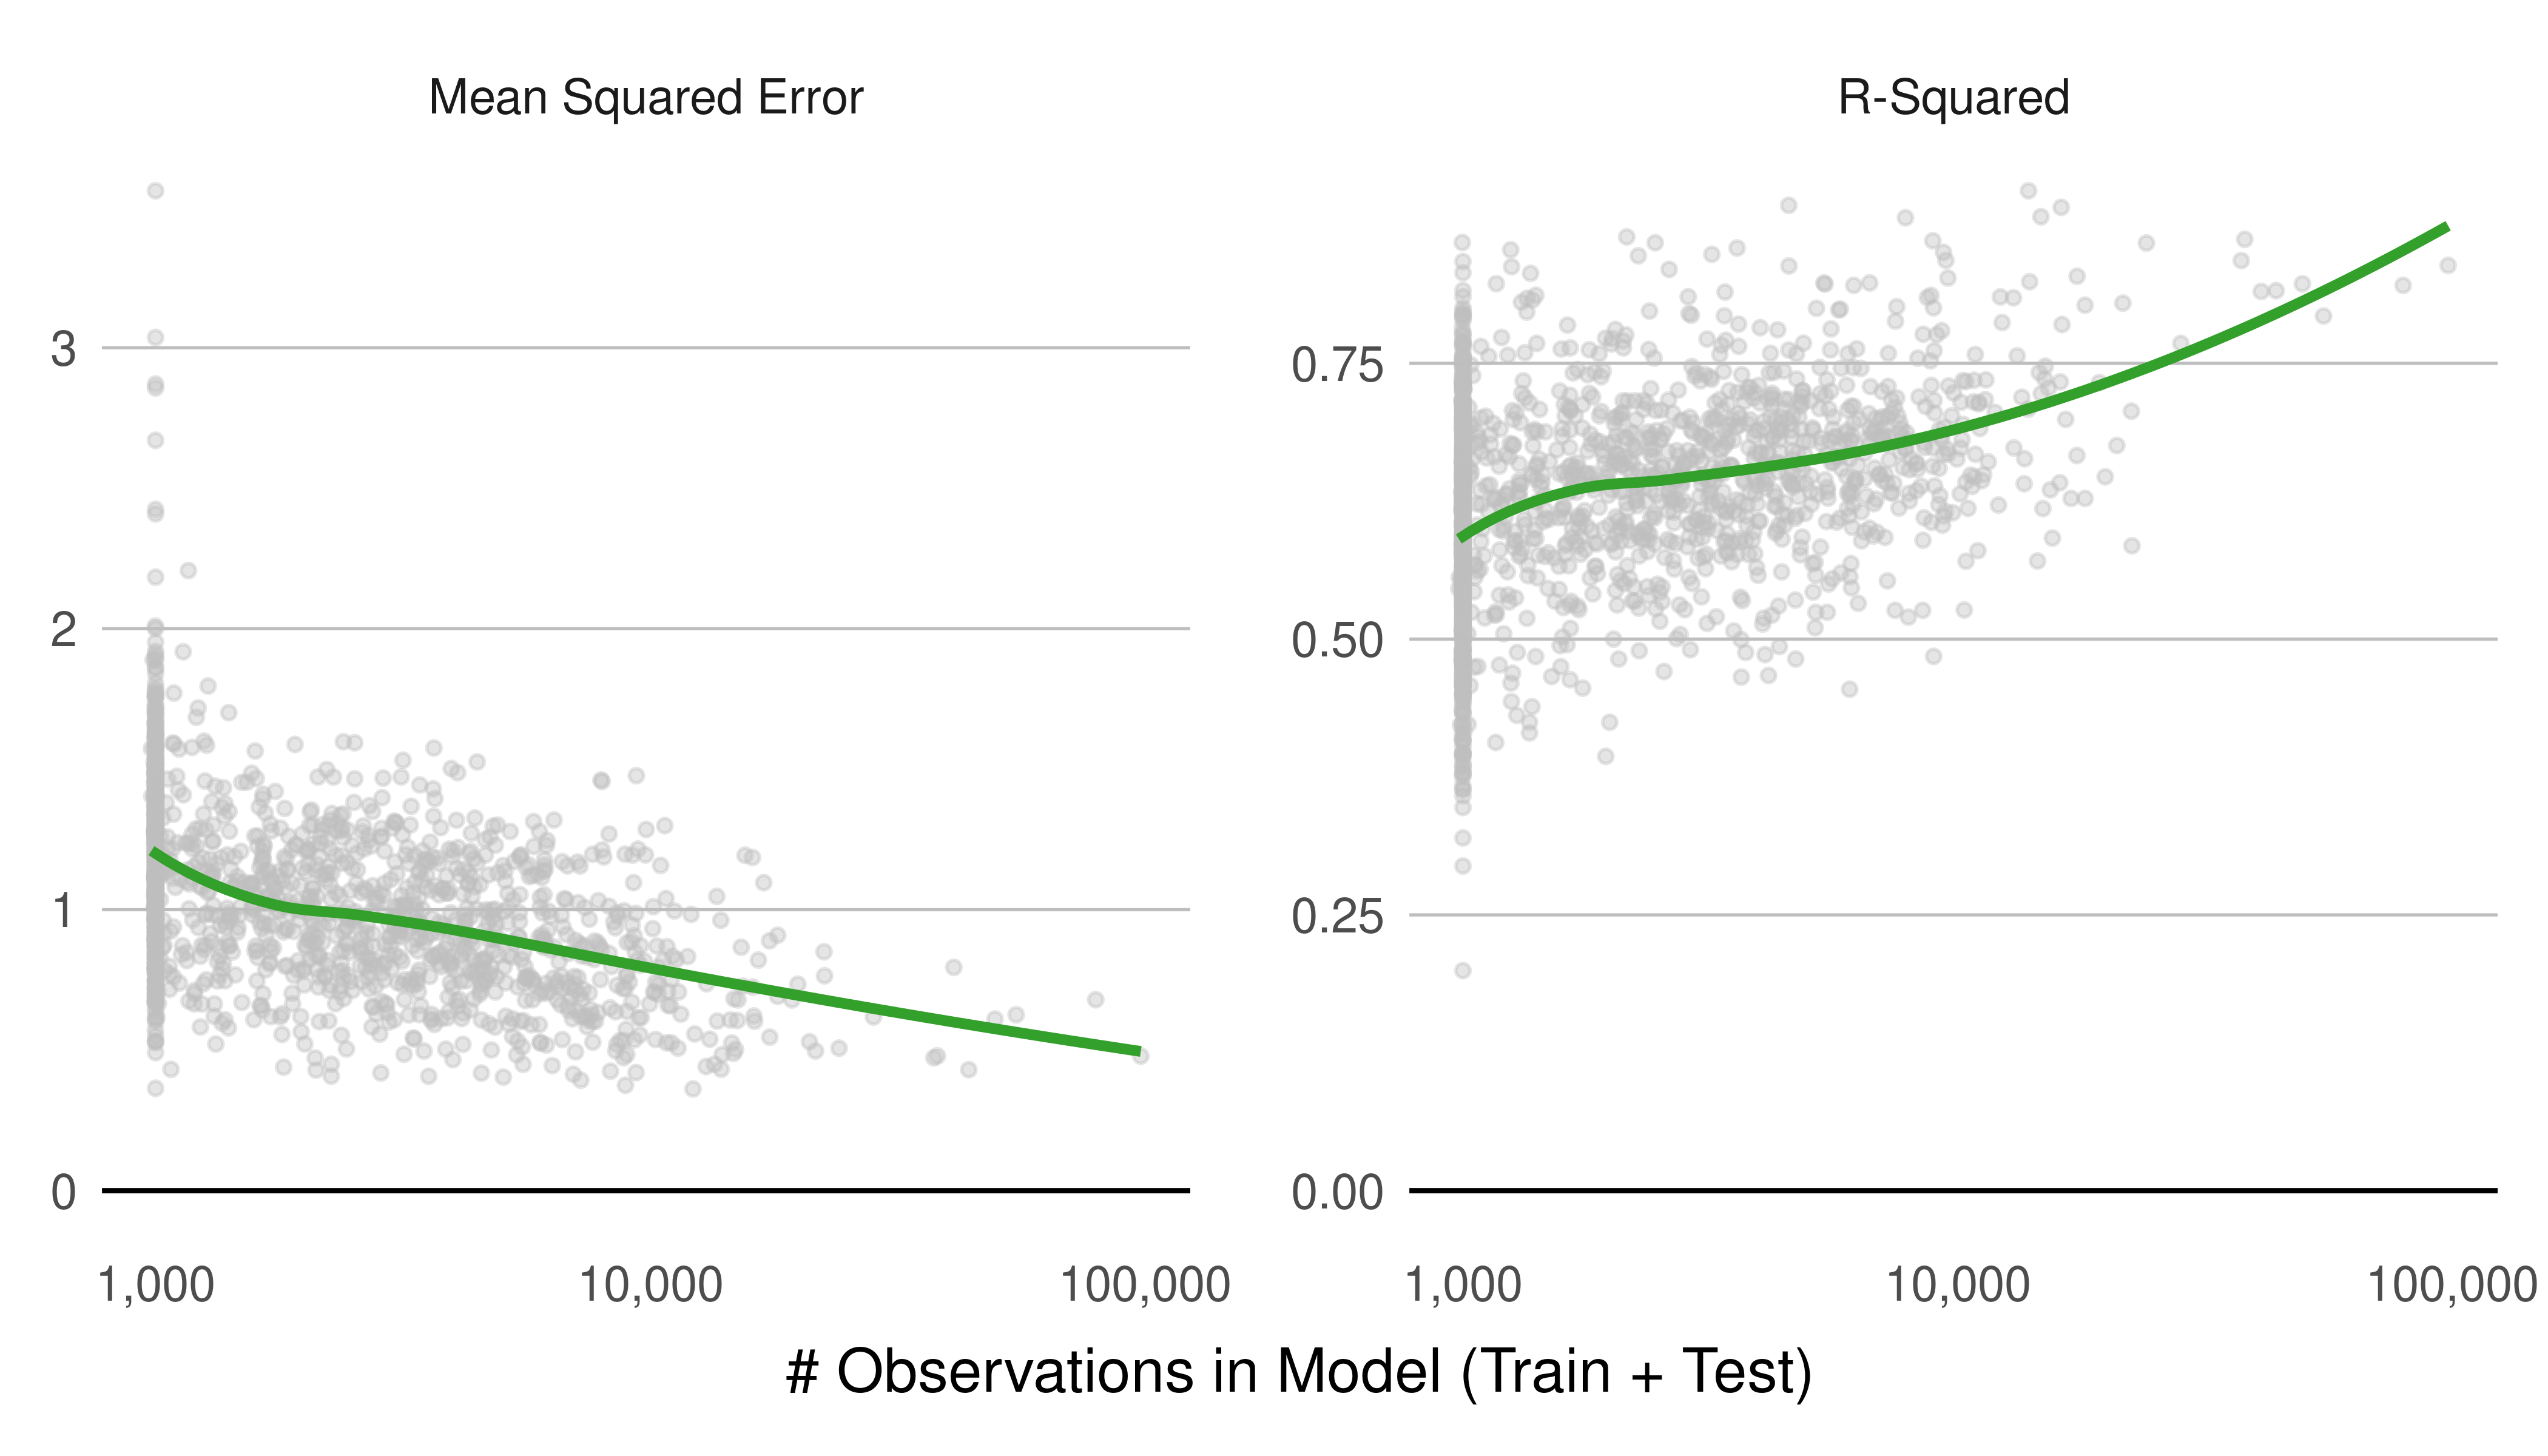
\includegraphics[width=1\textwidth]{exhibits/compare_county_nobs_perf.png}
    \caption{Restricted county model performance across total county-level observations.}
    \label{fig:compare_county_nobs_perf}
\end{figure}

\begin{figure}[H]
    \centering
    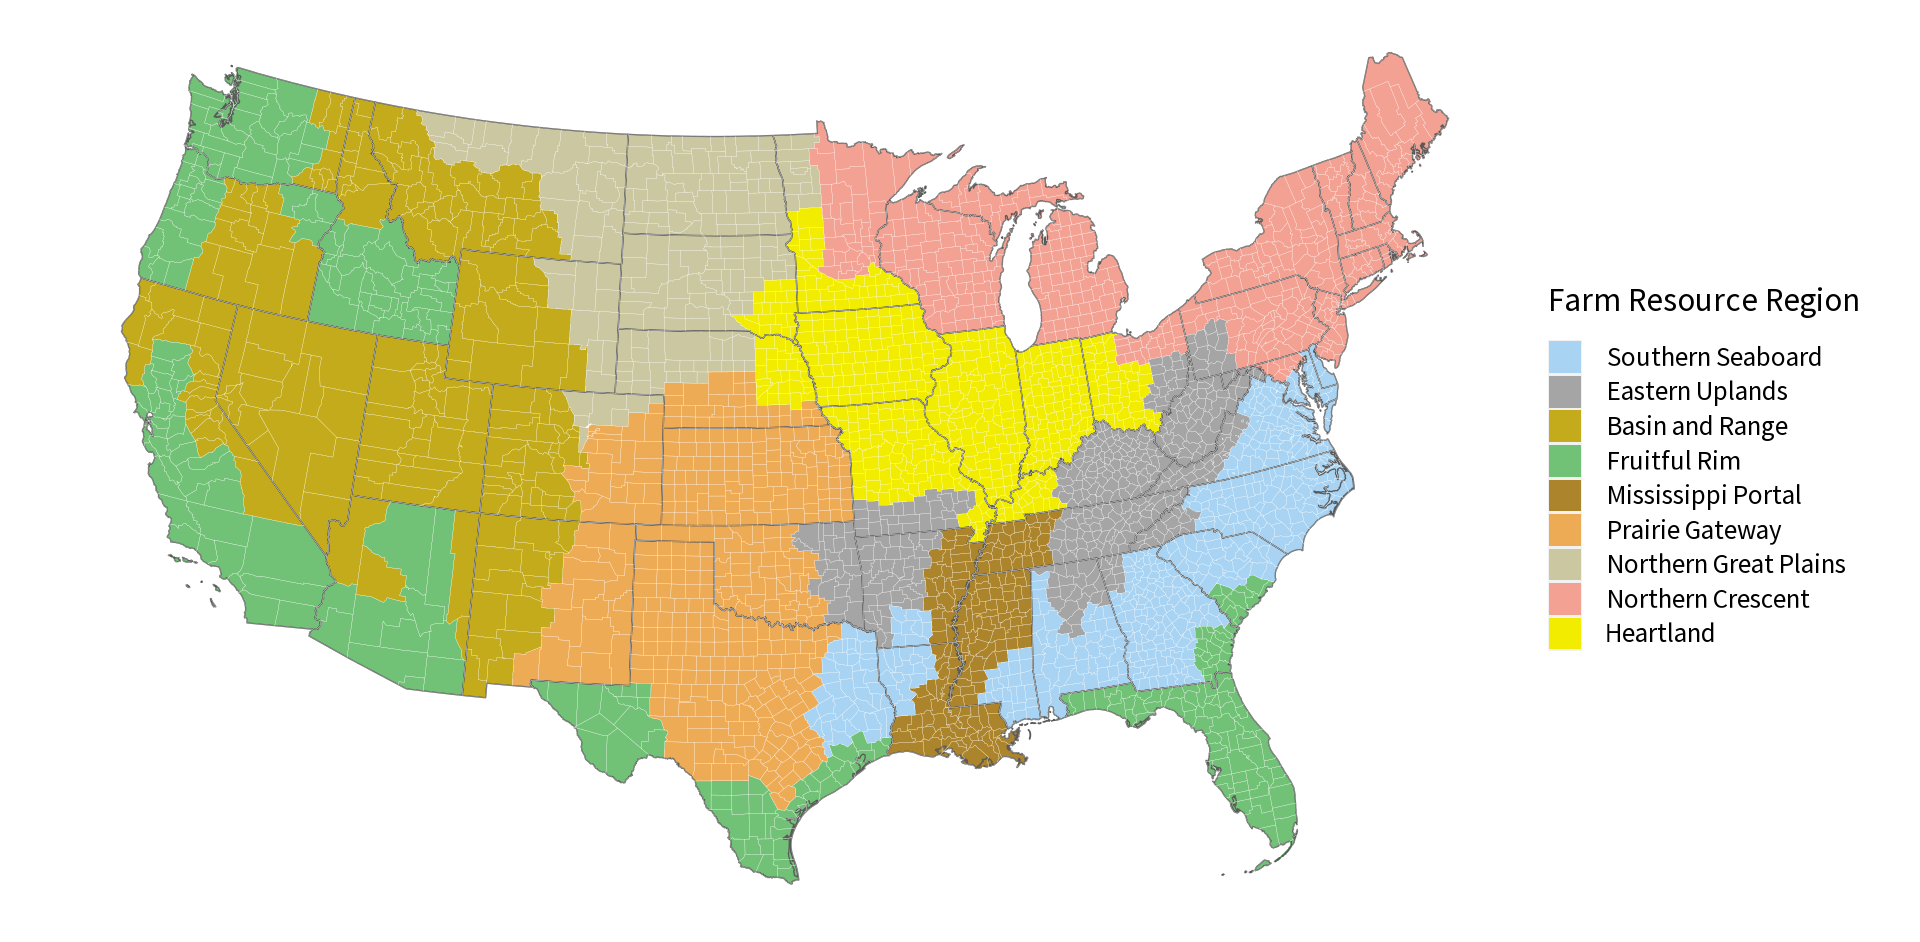
\includegraphics[width=1\textwidth]{exhibits/FRR_map.png}
    \caption{USDA Farm Resource Regions}
    \label{fig:FRR_map}
\end{figure}

\begin{figure}[H]
    \centering
    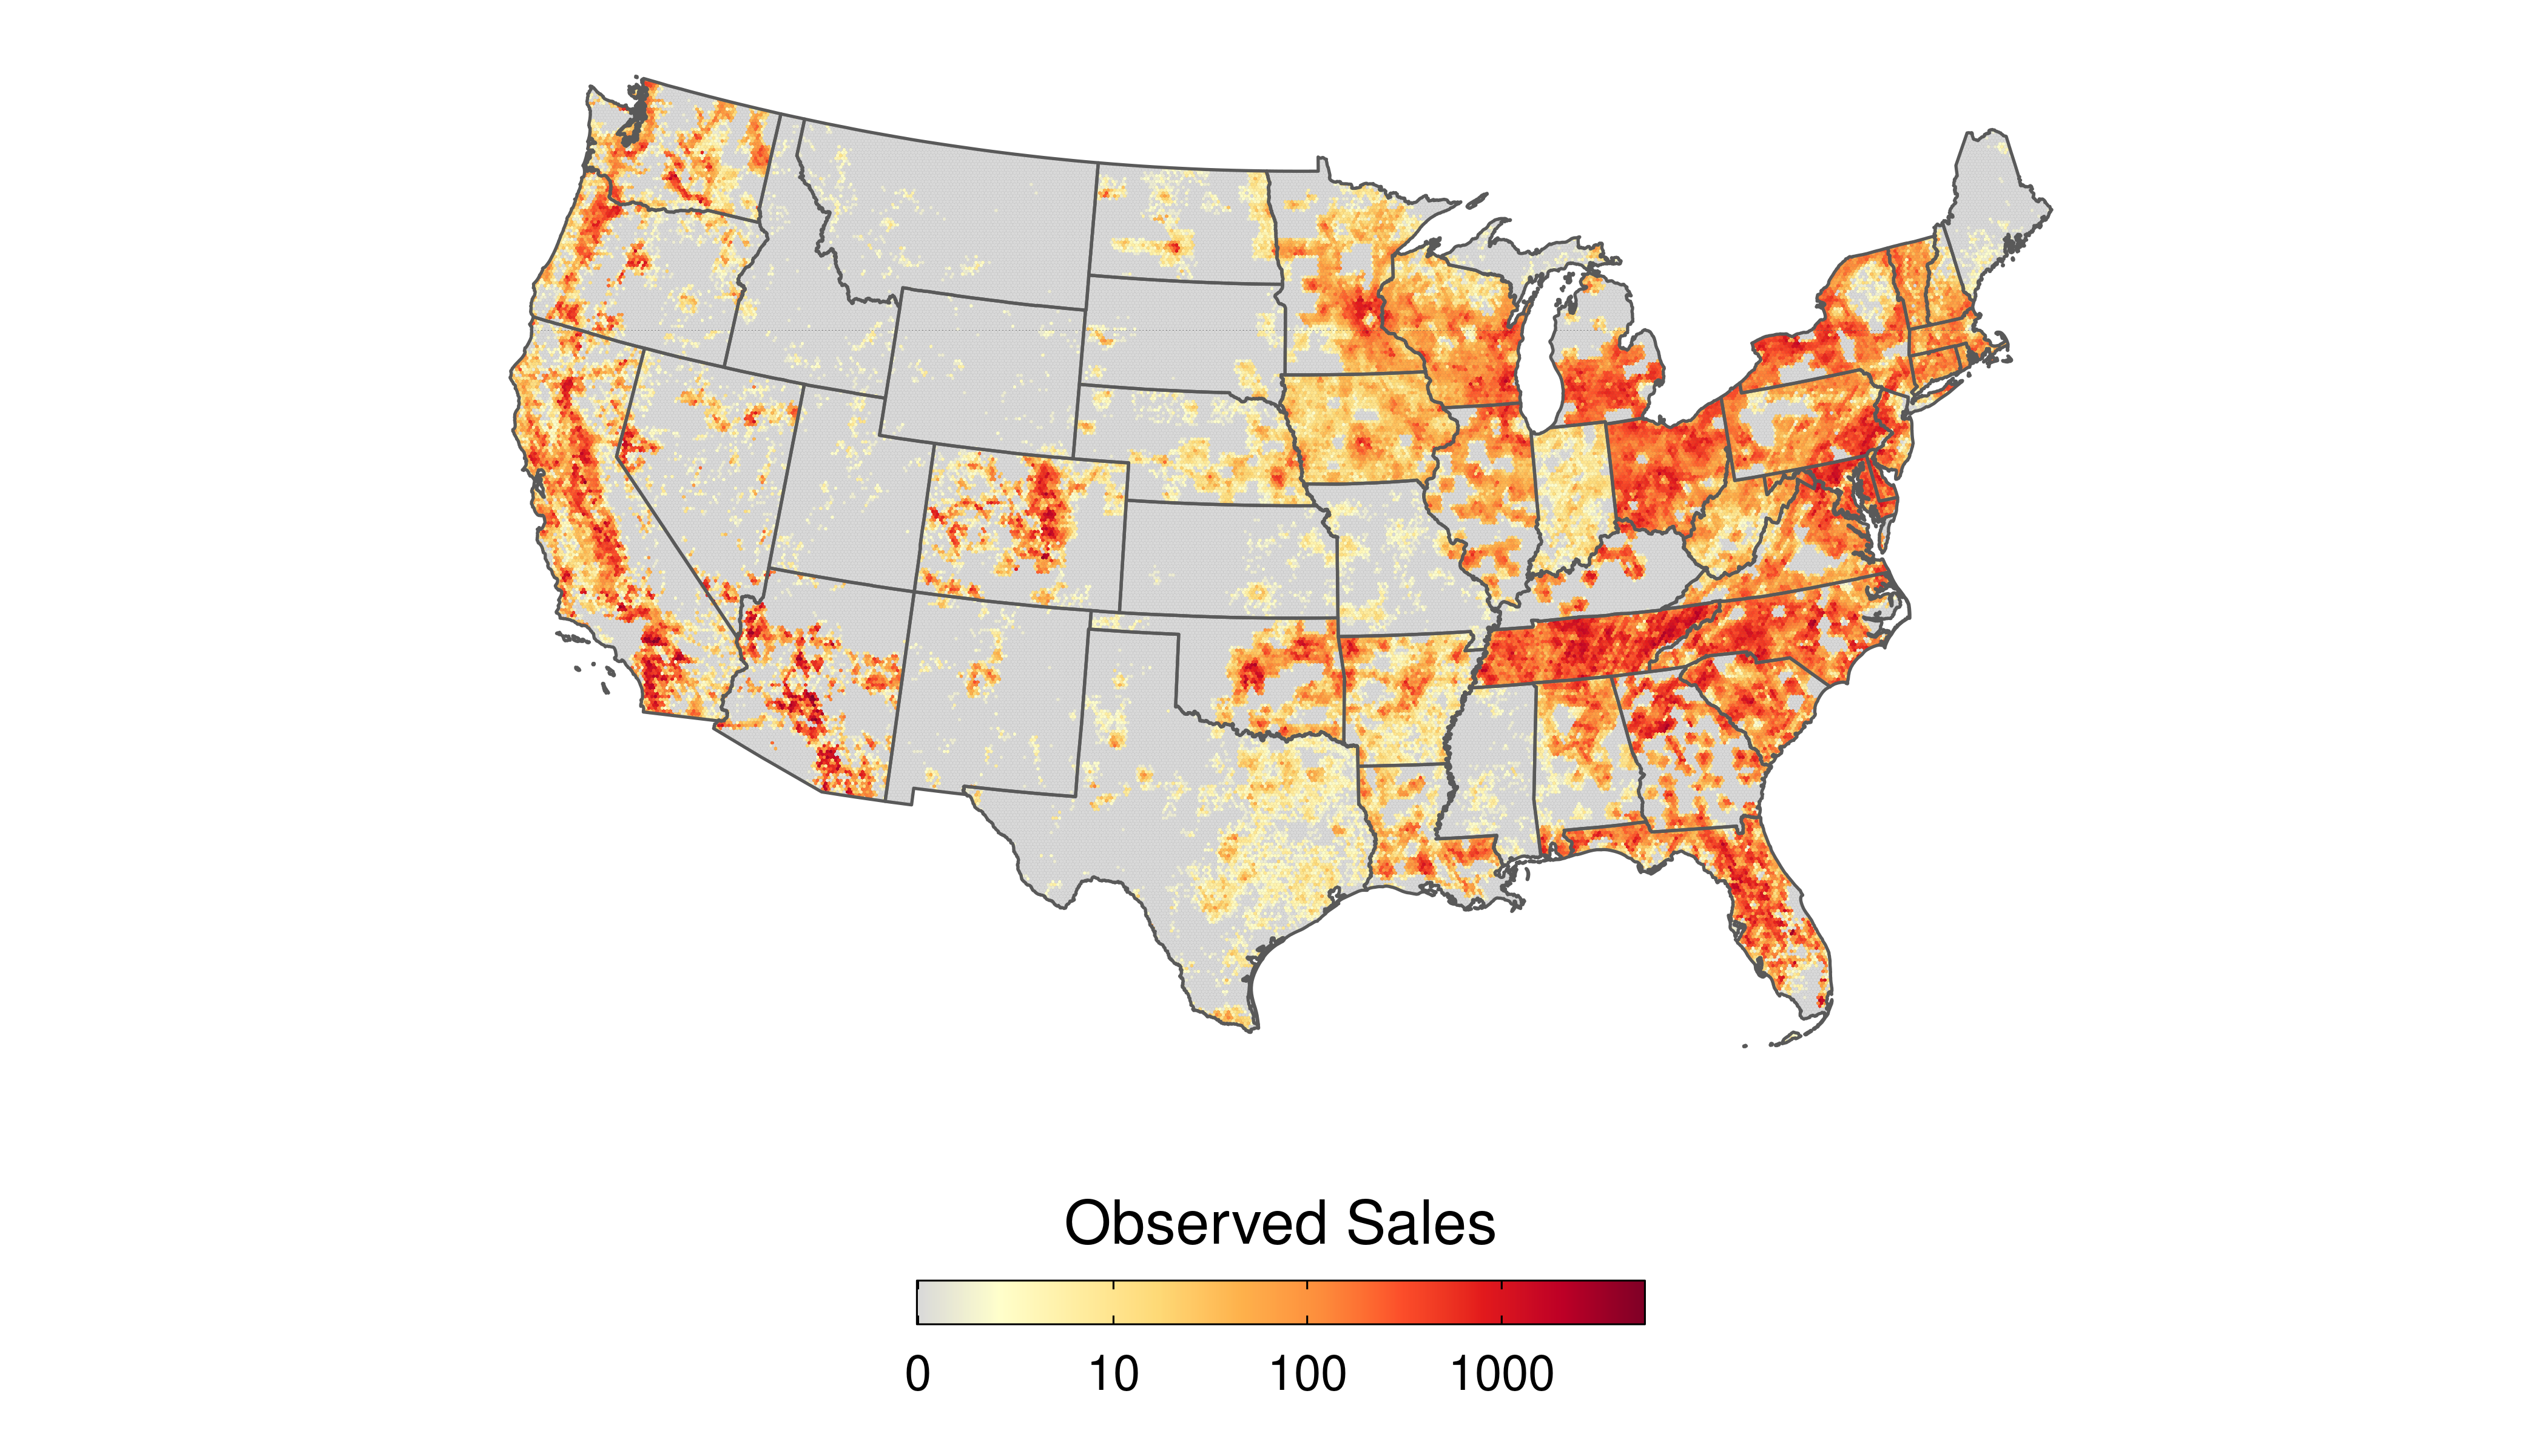
\includegraphics[width=1\textwidth]{exhibits/clean_obs_density.png}
    \caption{Spatial distribution of sales observations, 2000-2020, in filtered dataset. N = 5.04 million. Cells represent 10 km$^2$ tessellation of the conterminous US.}
    \label{fig:clean_obs_density}
\end{figure}

\begin{figure}[H]
    \centering
    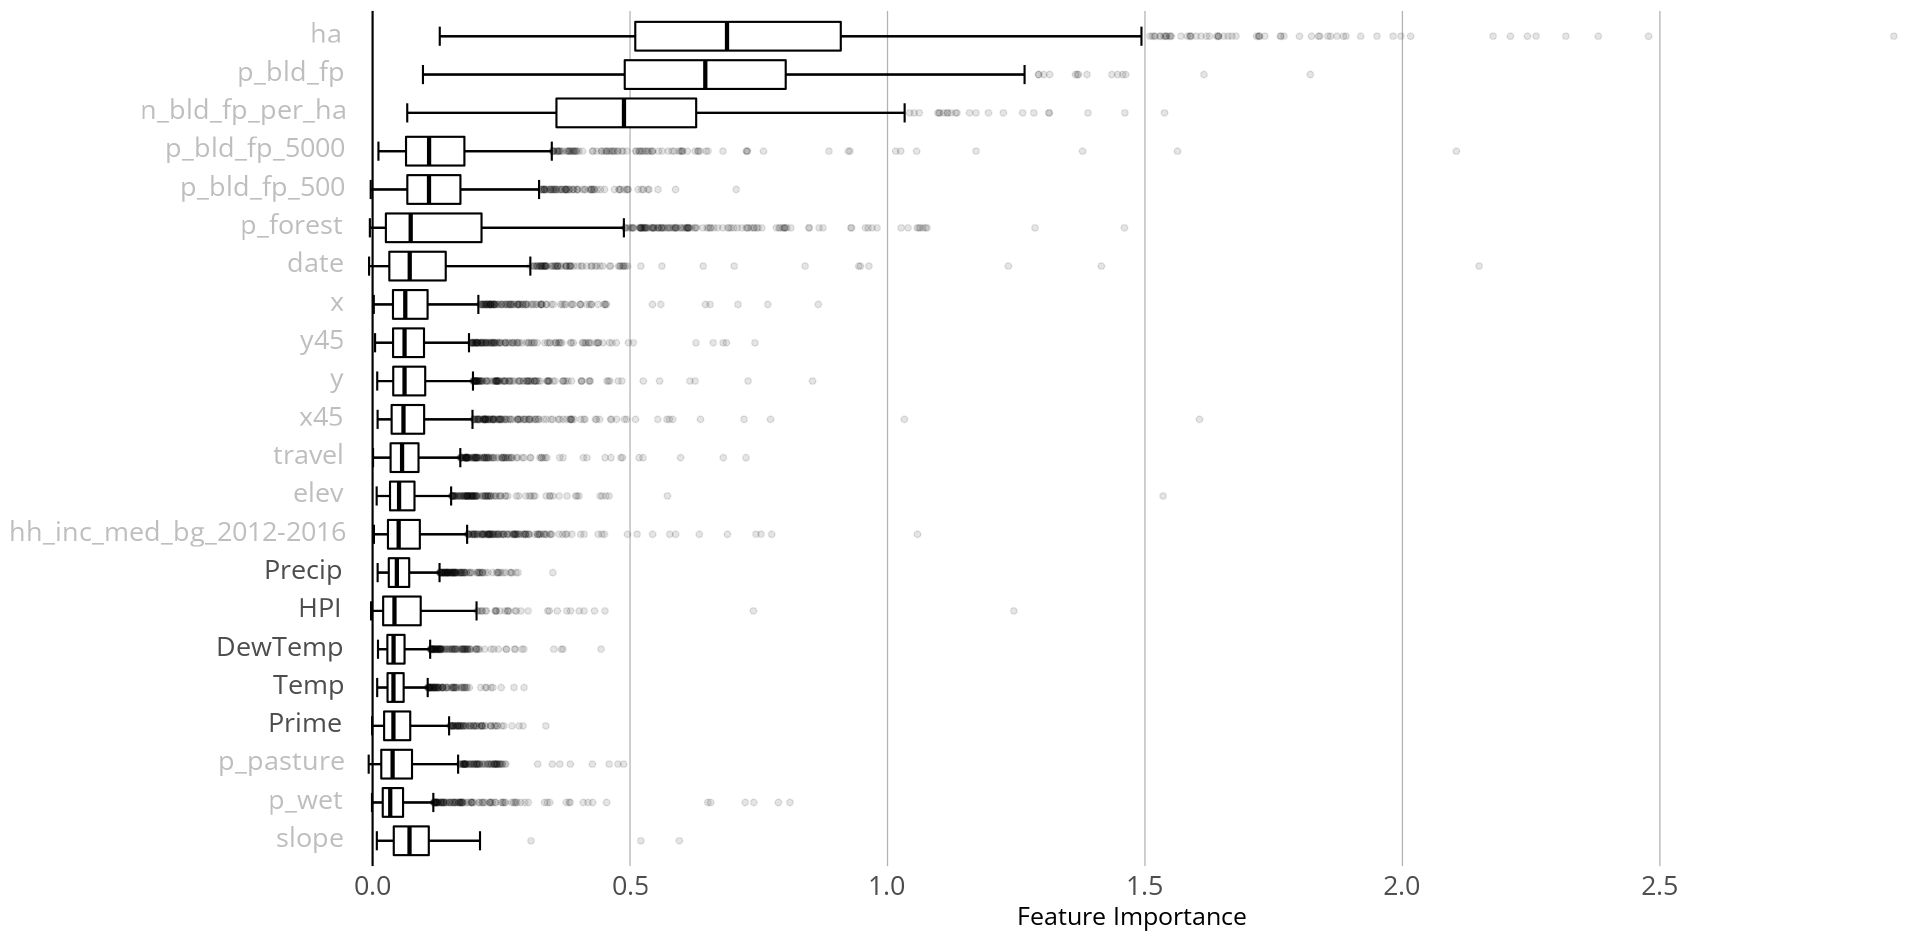
\includegraphics[width=1\textwidth]{exhibits/fcb_importance_t20.png}
    \caption{Permutation feature importance from full county model, top 20 features. Climatic variables grouped for clarity. Features added by this paper denoted in bold. Each dot represents a single county.}
    \label{fig:fcb_importance}
\end{figure}

\begin{figure}[H]
    \centering
    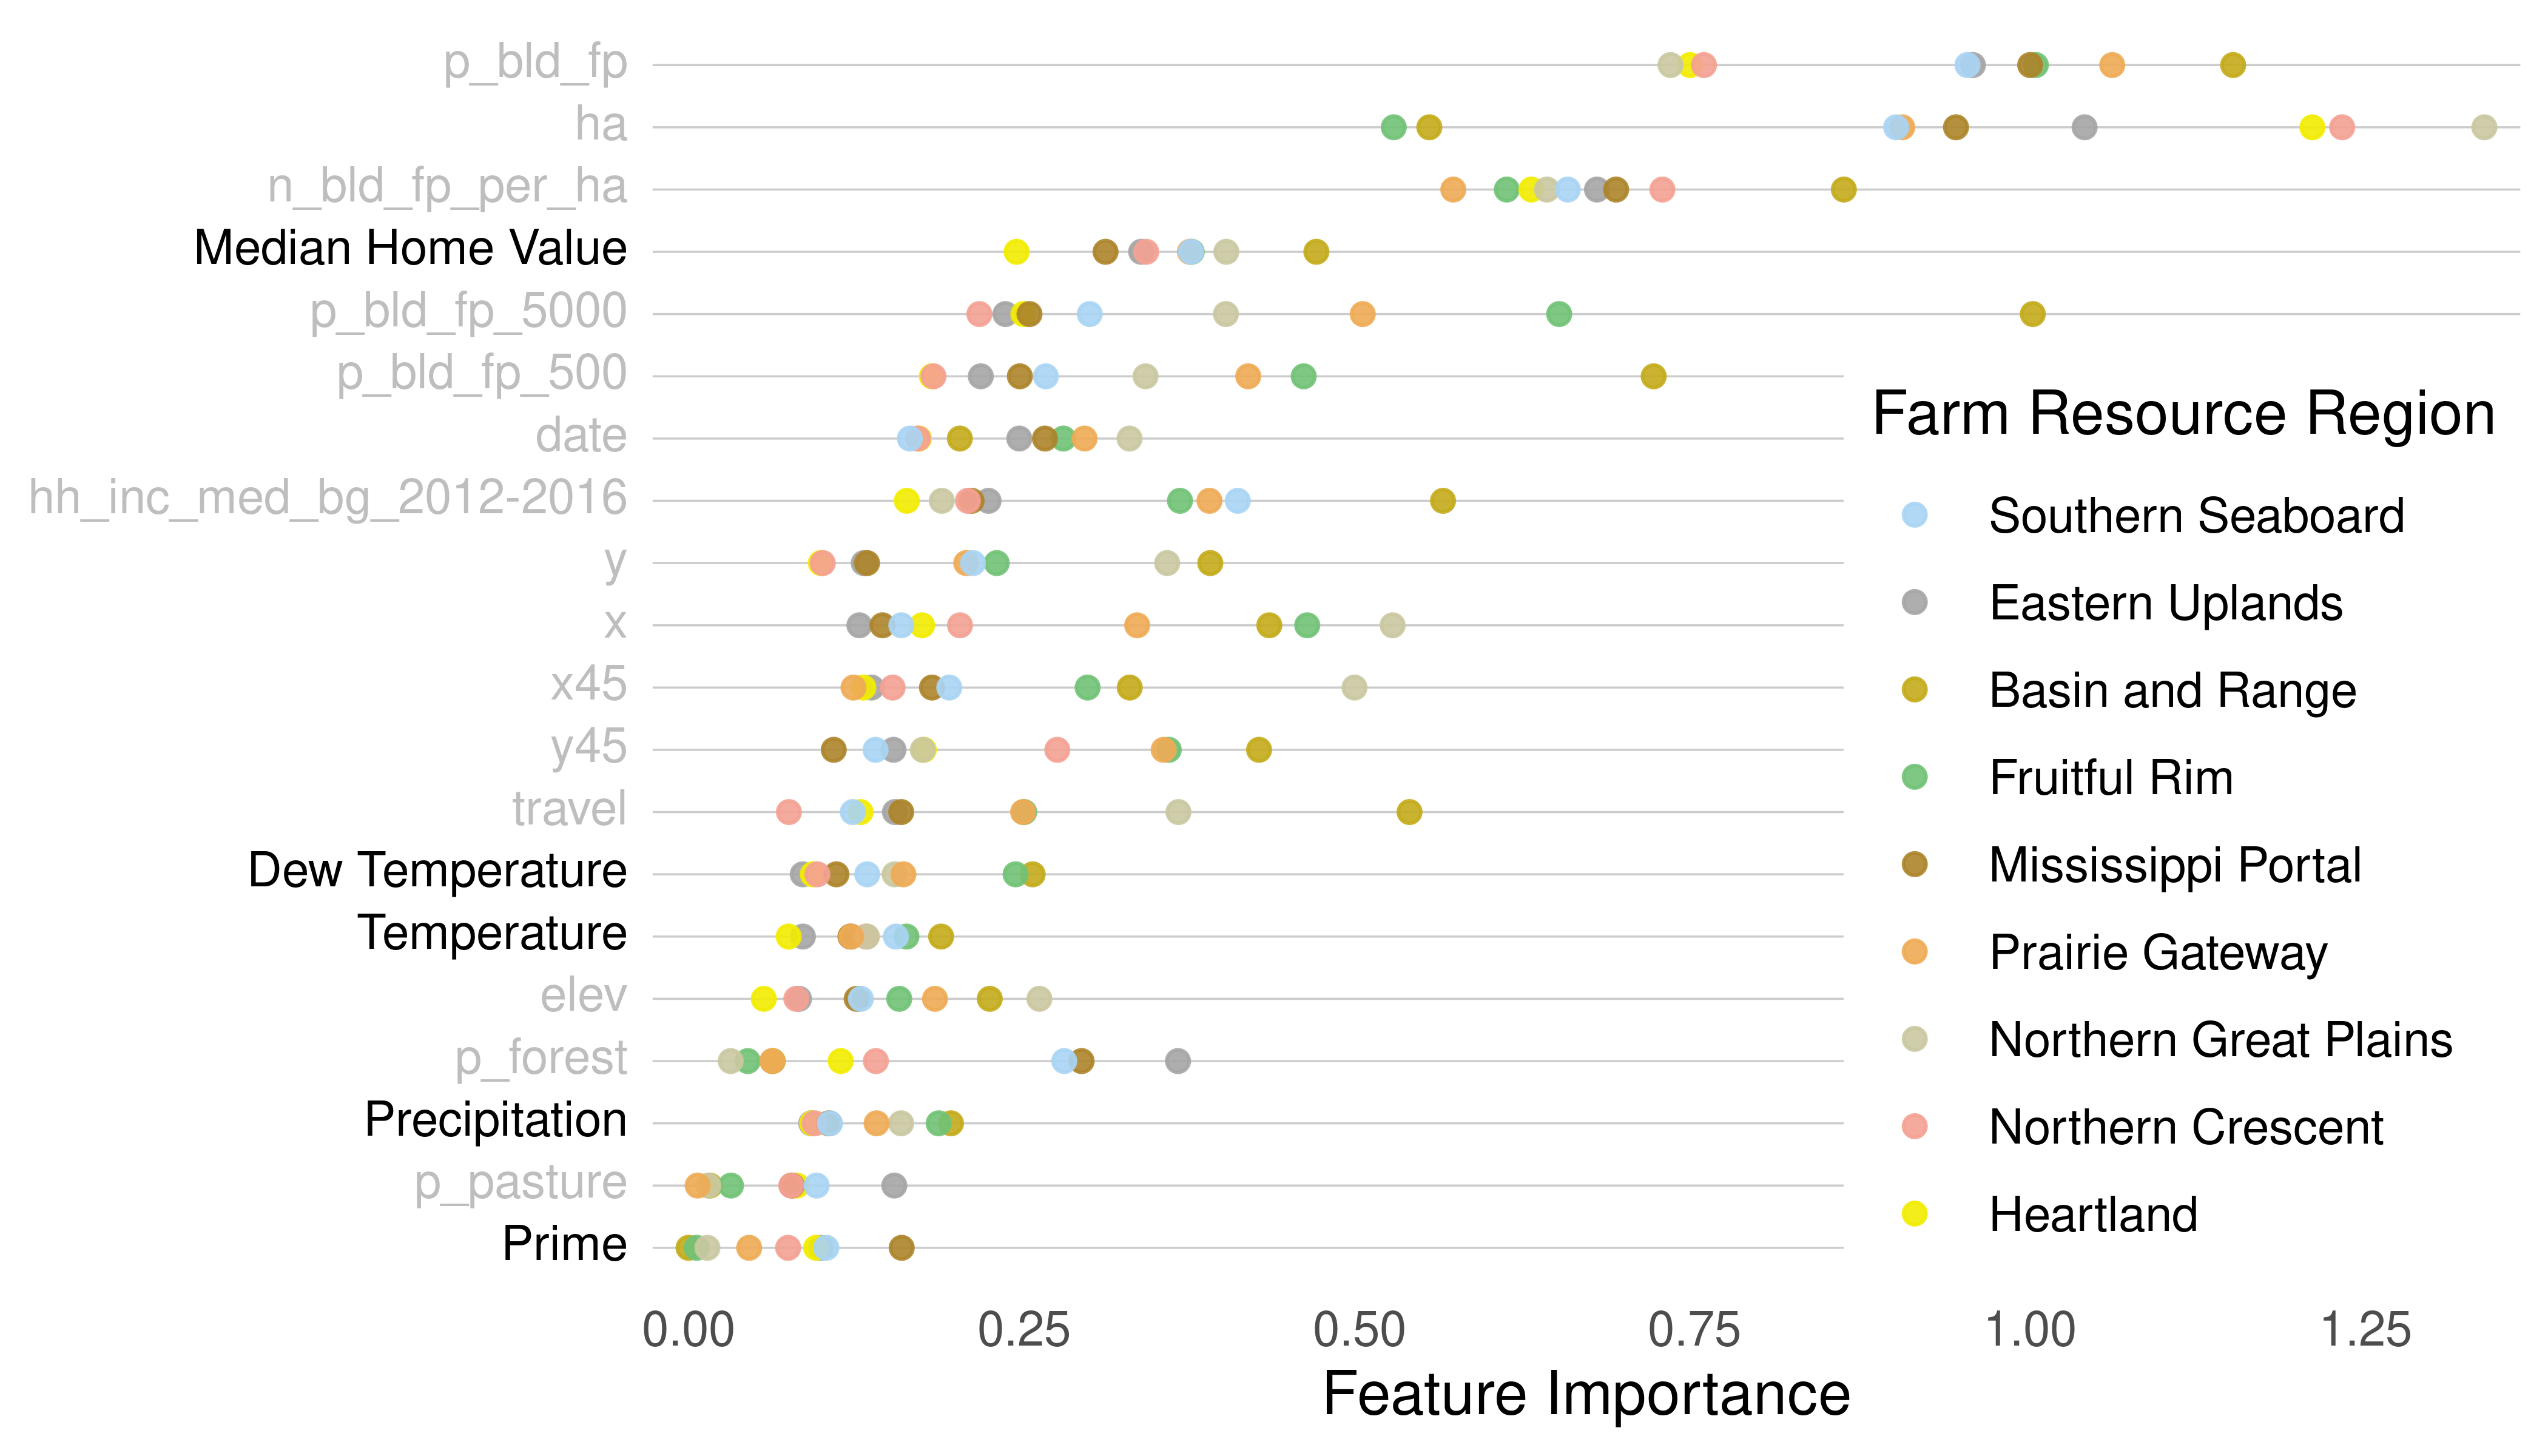
\includegraphics[width=1\textwidth]{exhibits/ffb_importance_t20.png}
    \caption{Permutation feature importance by farm resource region, top 20 features. Climatic variables grouped for clarity. Features added by this paper denoted in bold.}
    \label{fig:ffb_importance}
\end{figure}

\begin{figure}[H]
    \centering
    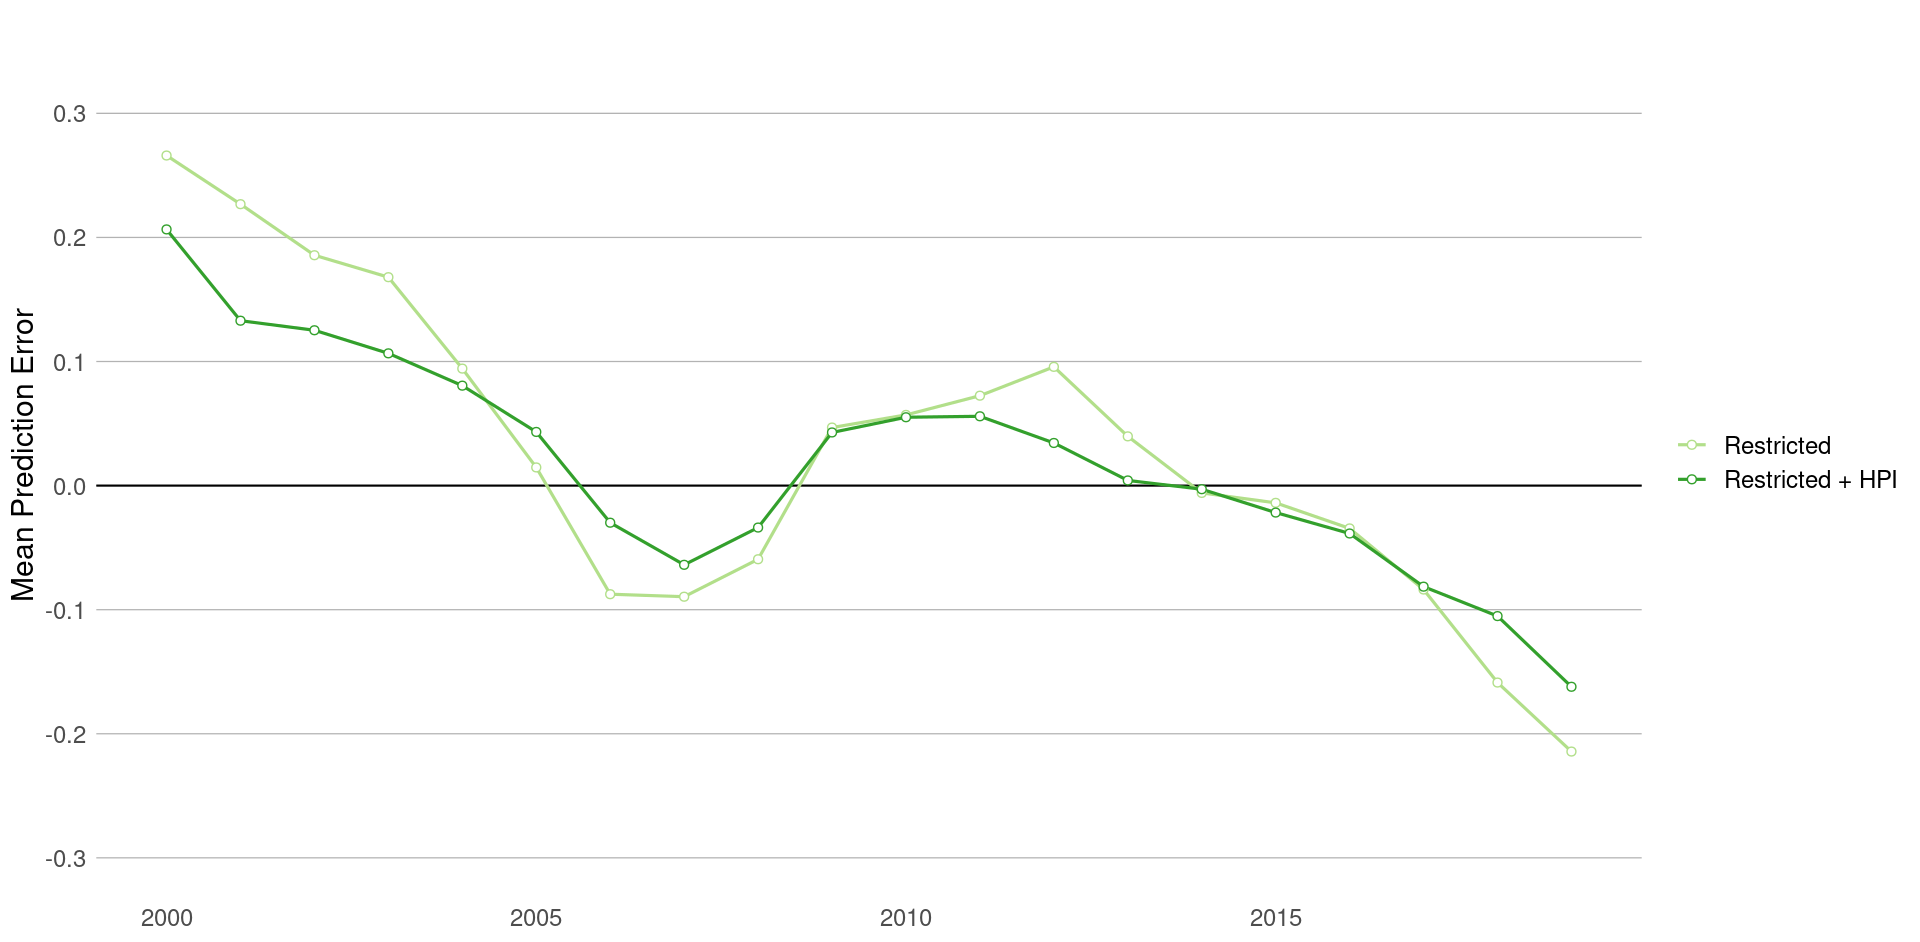
\includegraphics[width=1\textwidth]{exhibits/nolte_resid_time.png}
    \caption{Mean annual prediction error in Restricted county model, compared to the addition of annual housing price index data at the county level.}
    \label{fig:nolte_resid_time}
\end{figure}

\begin{figure}[H]
    \centering
    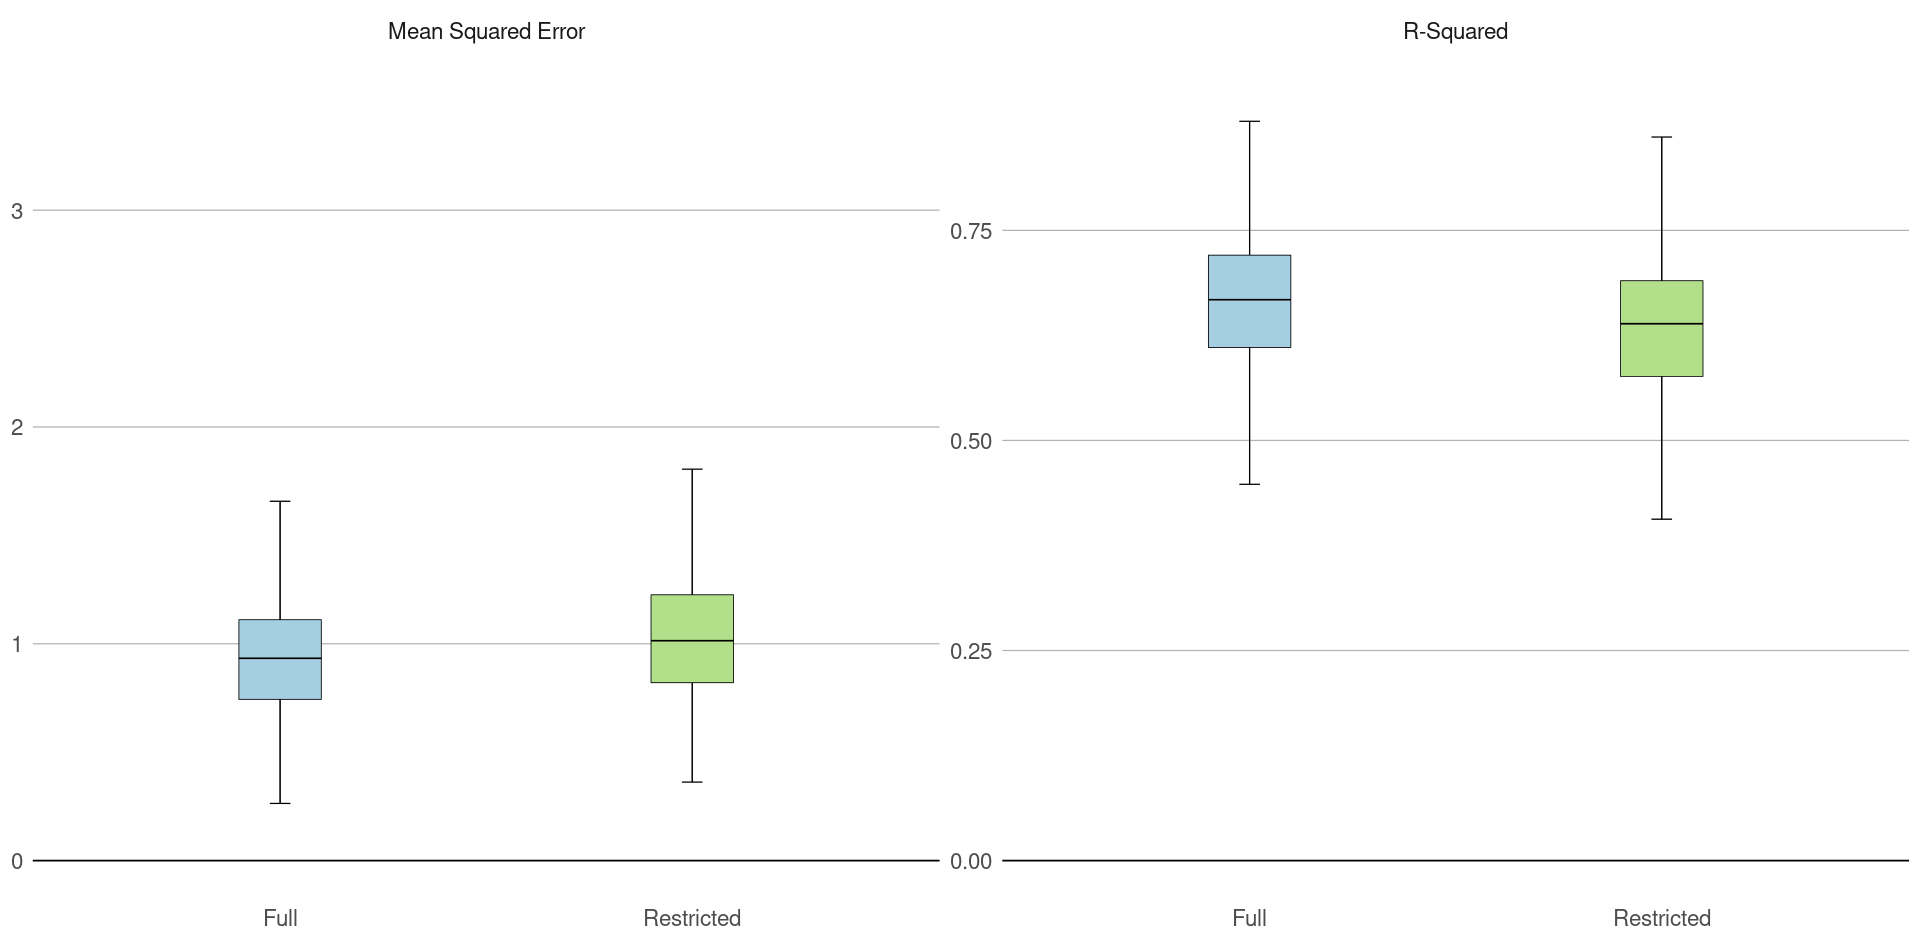
\includegraphics[width=1\textwidth]{exhibits/county_compare_boxplot.png}
    \caption{County-level model performance, Full compared to Restricted. Outliers removed for clarity.}
    \label{fig:county_compare_boxplot}
\end{figure}

\begin{figure}[H]
    \centering
    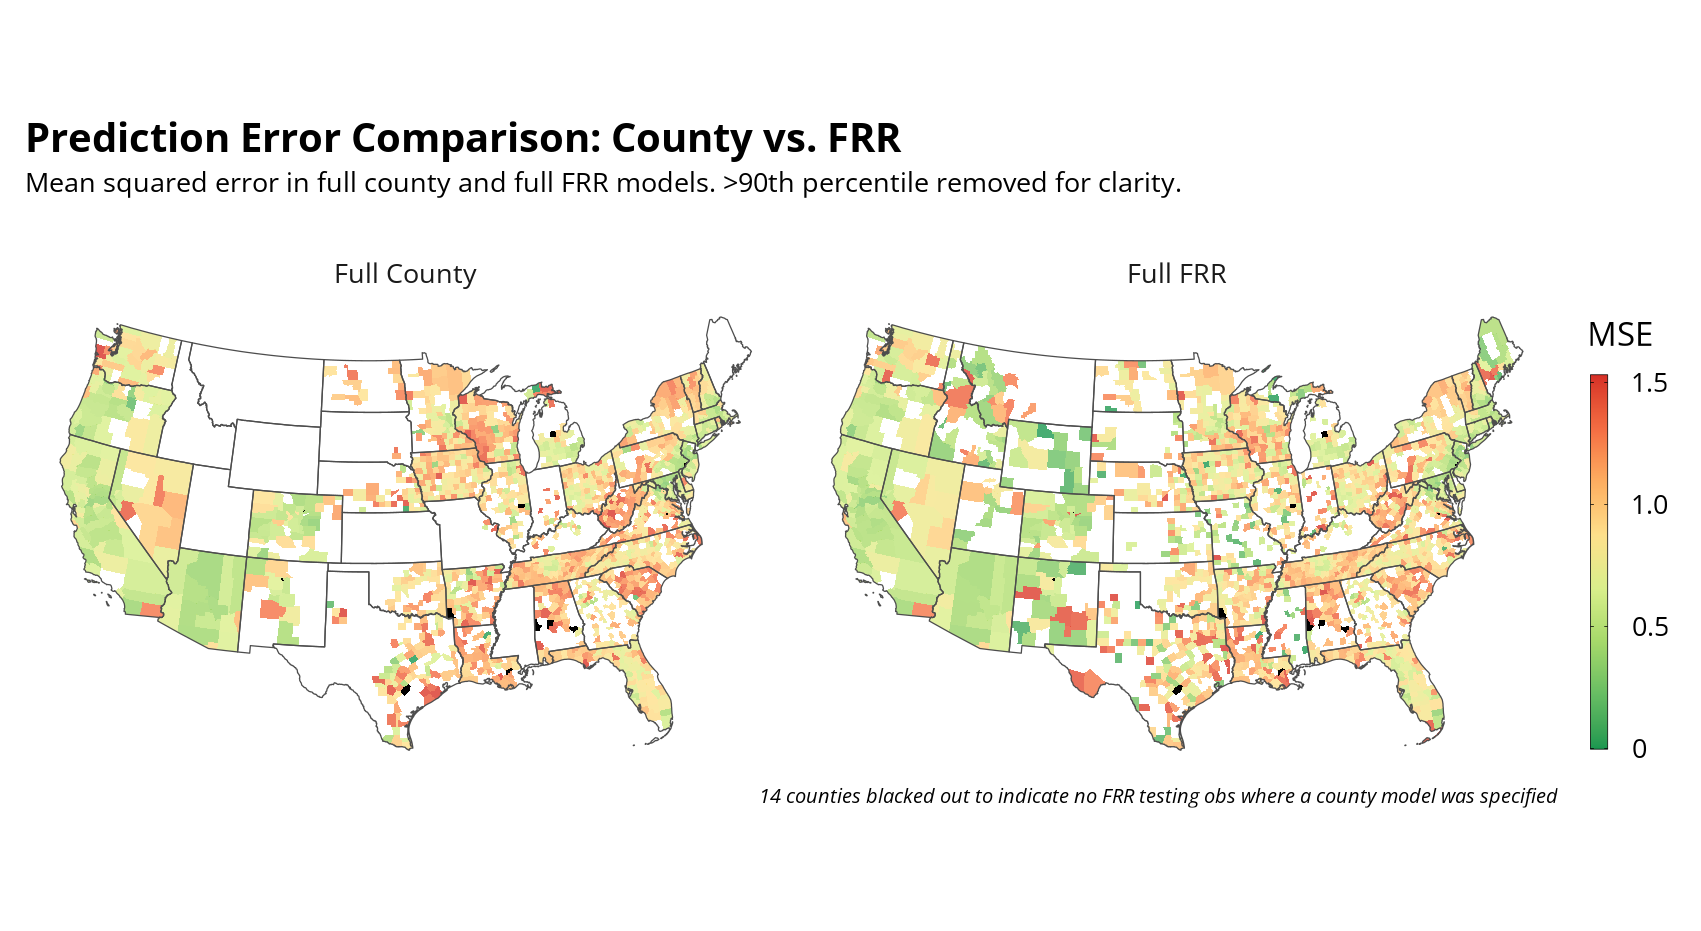
\includegraphics[width=1\textwidth]{exhibits/compare_ffb_fcb_mse.png}
    \caption{Mean squared error in Full county model (left) and Full farm resource region model (right). Counties with MSE greater than the 90th percentile have been removed for visual clarity. Blacked-out counties indicate 14 instances wherein a county model was specified but the farm resource region model did not include testing observations in that county.}
    \label{fig:compare_ffb_fcb_mse}
\end{figure}

\begin{figure}[H]
    \centering
    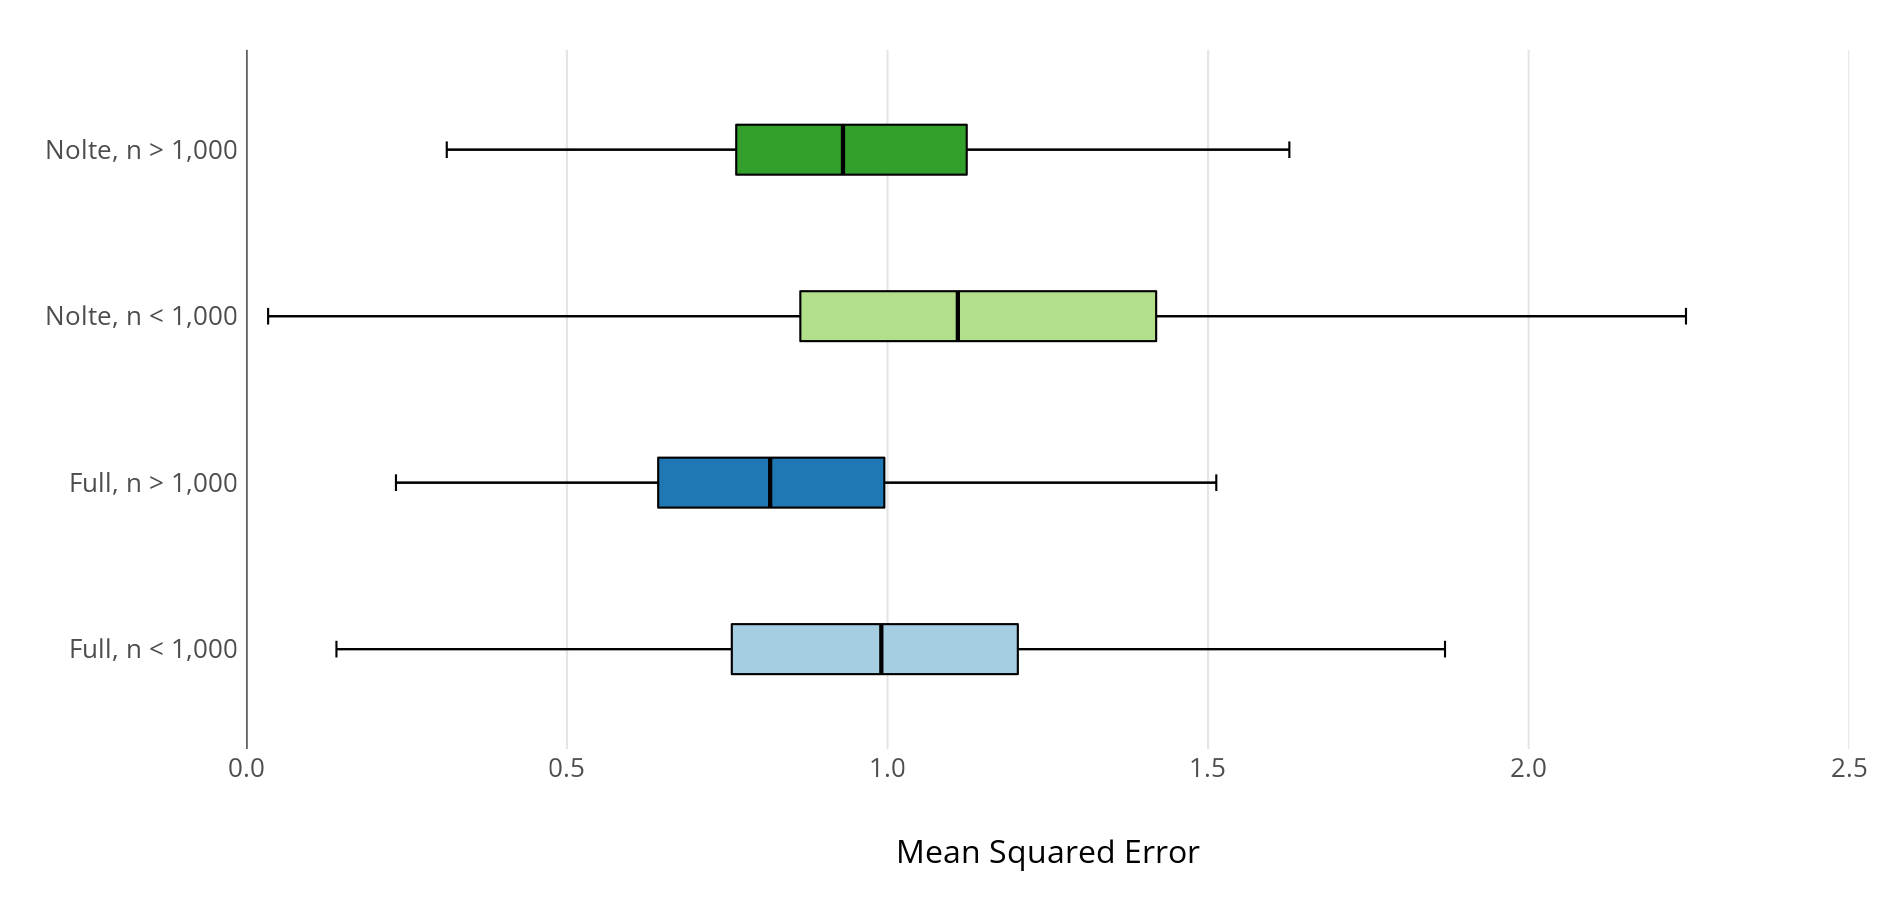
\includegraphics[width=1\textwidth]{exhibits/frr_compare_mse_size.png}
    \caption{Average county-level mean squared error in farm resource region models by size category, Restricted compared to Full. Outliers removed for clarity.}
    \label{fig:frr_compare_mse_size}
\end{figure}



\newpage
\newpage

\vspace*{200pt}

\begin{huge}
    \begin{center}
        Appendix
    \end{center}
\end{huge}

\newpage

\subsection*{A.1 Parcel filter}

\begin{enumerate}
    \item Meets ``undeveloped" criteria established by Nolte (2020), \textbf{or}
    \item Over half its area was classified as either grassland/herbaceous or planted/cultivated in the 2011 National Land Cover Database (NLCD), \textbf{or}
    \item Over half its area was classified as agricultural in the 2000 Land Change Monitoring, Assessment, and Projection (LCMAP), \textbf{or}
    \item Had any of the following ZTRAX land use codes:
    \begin{enumerate}
        \item Agricultural (``AG");
        \item Homestead (``MS113");
        \item Vacant open space/conservation/forest land (``VL104");
        \item Vacant agricultural/unimproved (``VL108")
    \end{enumerate}
\end{enumerate}

\newpage

\subsection*{A.2 Feature Importance: All Features}


\begin{figure}[H]
    \centering
    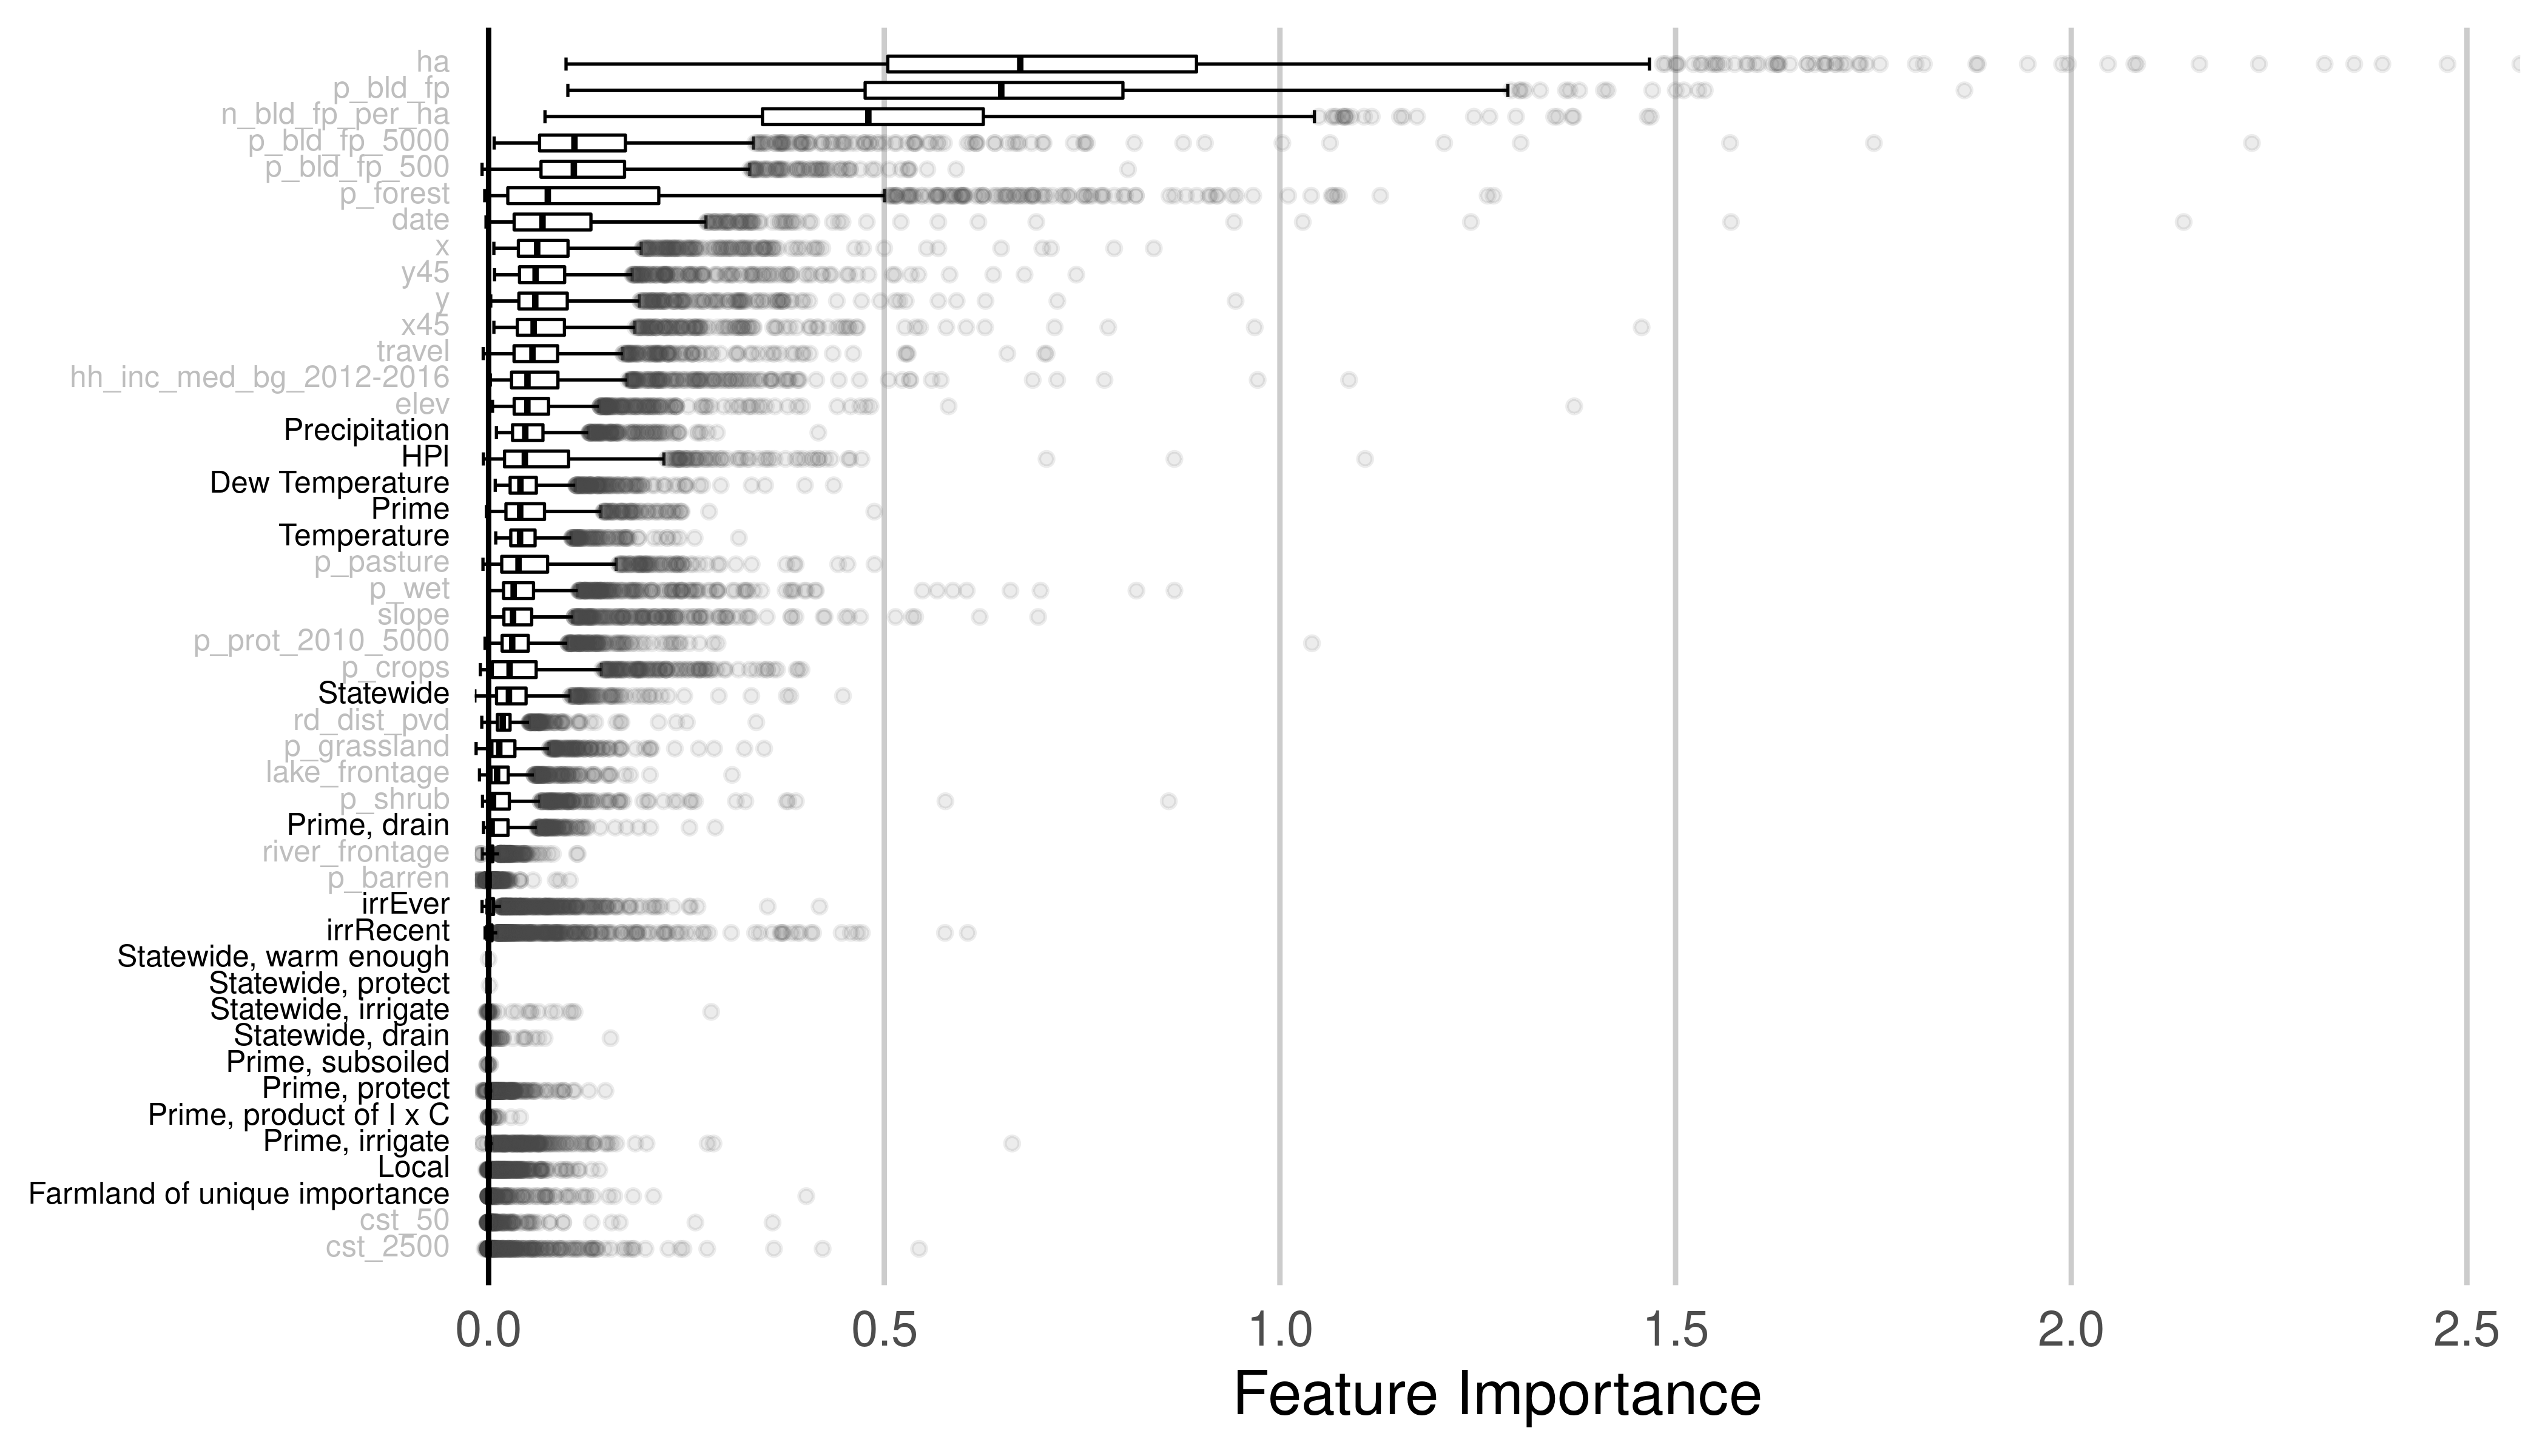
\includegraphics[width=0.9\textwidth]{exhibits/fcb_importance_all.png}
    \caption{Permutation feature importance from full county model, all features. Climatic variables grouped for clarity. Features added by this paper denoted in bold. Each dot represents a single county.}
    \label{fig:fcb_importance_all}
\end{figure}

\begin{figure}[H]
    \centering
    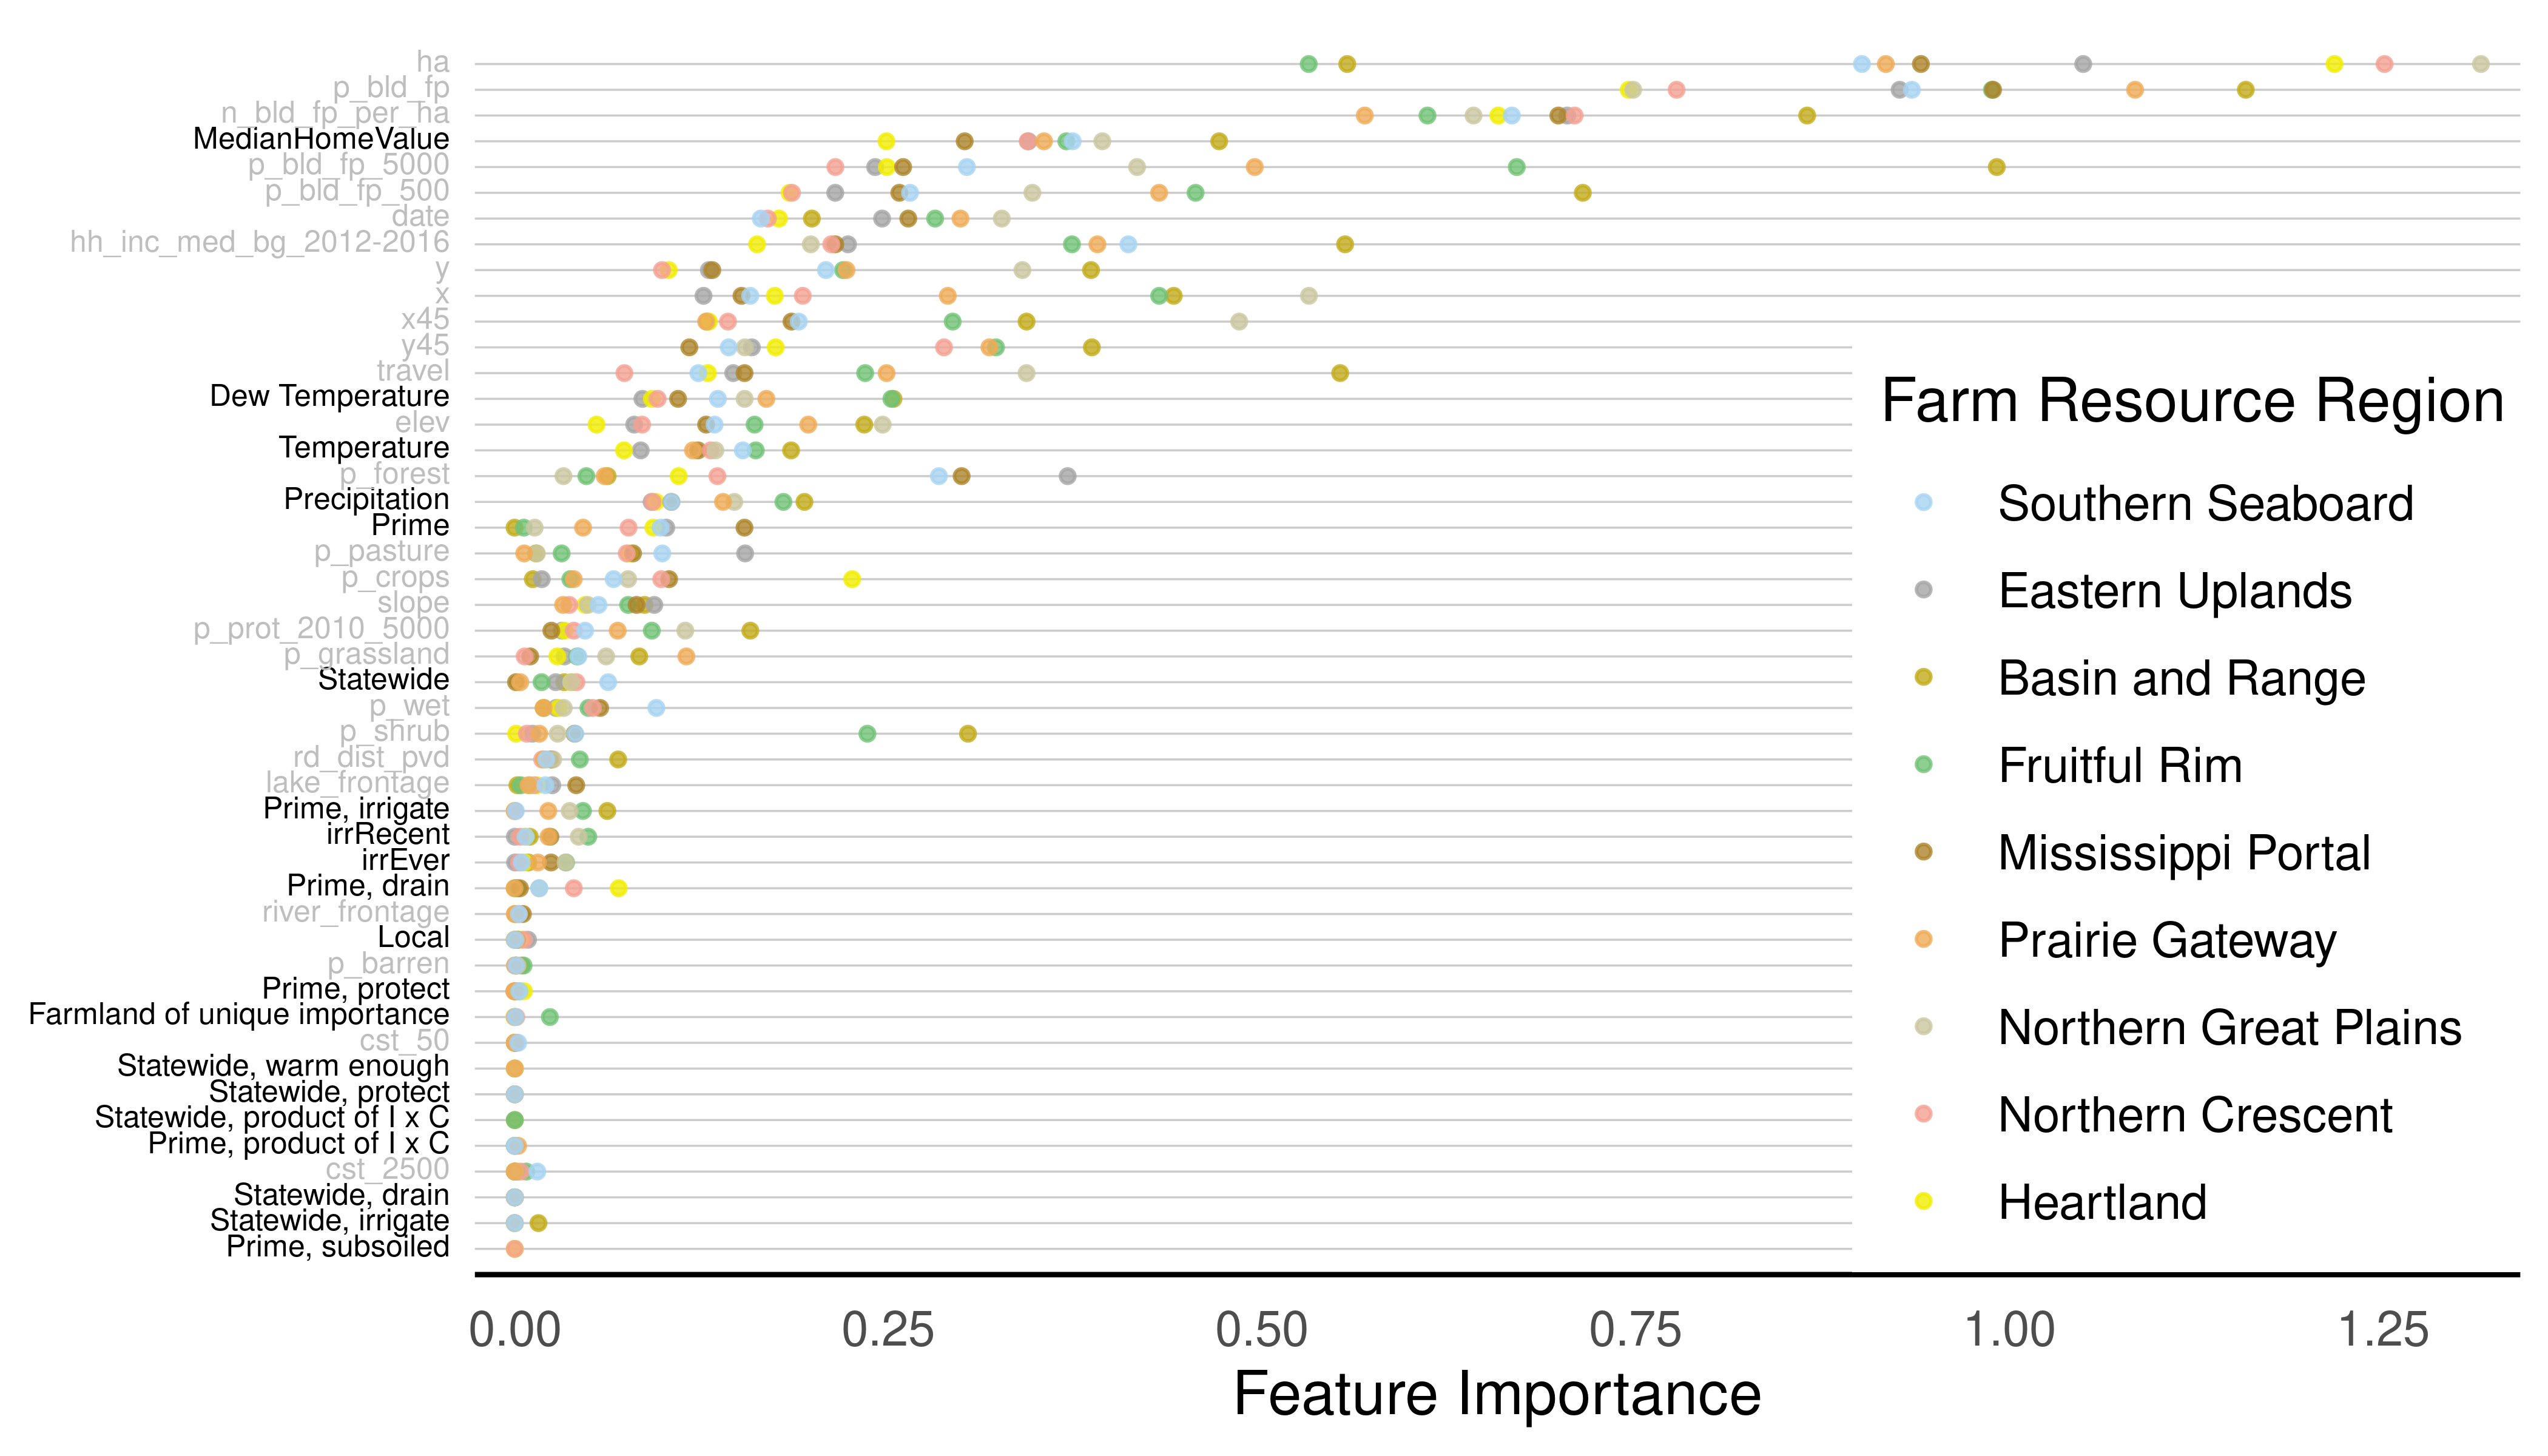
\includegraphics[width=0.9\textwidth]{exhibits/ffb_importance_all.png}
    \caption{Permutation feature importance by farm resource region, all features. Climatic variables grouped for clarity. Features added by this paper denoted in bold.}
    \label{fig:ffb_importance_all}
\end{figure}

\newpage

\subsection*{A.3 Multi-parcel Aggregation}
Our analysis employs sales as the individual sample unit. In the case of sales involving multiple parcels, we aggregate predictor values across sales. 

We take the arithmetic mean of all Nolte (2020) variables except river and lake frontage length, which we sum across all parcels.

For all climatic variables added by this paper (precipitation, dew temperature, and temperature), we take the hectare-weighted mean across all parcels.

For irrigation indicator variables (ever irrigated and irrigated in the past three years), we take the maximum of all parcels' indicators. If any parcel in the sale has been irrigated, the sale is considered irrigated.

For soil types, we calculate a given soil type j's proportion $p_j$ as the proportion of total soil area across each parcel $i$ occupied by that soil type:

\[
p_j = \displaystyle\frac{\sum\limits_{i=1}^{n}p_{j,i}}{\sum\limits_{i=1}^{n}area_i}
\]


\newpage


\printbibliography

\end{document}